%*******************************************************************************
%****************************** Second Chapter *********************************
%*******************************************************************************

\chapter{Resultados Capítulo 2} 
{\LARGE Estudios genómicos sobre la biogénesis de miARN en plantas}

\graphicspath{{Chapter2/Figs/}}

\section{Introducción}
Los miARNs son una clase de ARNs de 20-22nt de largo que son originados de genes endógenos y regulan otros ARNs por complementariedad de bases \citep{Voinnet2009669}.
Se distinguen de otros ARNs pequeños por su biogénesis única que involucra el corte preciso del precursor, para liberar el miARN maduro.
Aunque la evidencia actual indica que los miARNs han surgido y especializada de forma independiente en animales y las plantas, su biogénesis depende del reconocimiento de claves estructurales ubicadas en los precursores de miARN \citep{pmid21554756,citeulike:8816489,Bologna11112012}.

En nuestro grupo actualmente se está estudiando la biogenesis de miARNs, específicamente como los precursores son reconocidos y procesados en plantas \citep{Bologna2013}.
Estos precursores tienen una estructura de tallo-burbuja característica \citep{Jones-Rhoades2006}, que se cree que proporciona las claves para el procesamiento del mismo y la liberación de los ARN pequeños de 21 nt.

Mientras que los precursores de miARN en animales tienen estructuras homogéneas, los precursores de miARNs en plantas constituyen una amplia gama de estructuras, y sus longitud pueden variar entre 50 y 900 nucleótidos \citep{Bologna2013,citeulike:8816489}.
Esa variabilidad se da entre distintas familias de precursores, pero a veces también entre una misma familia de precursores en distintas especies (Figura \ref{fig:hairpin_distribution}).

\begin{figure}[htbp!] 
    \centering    
    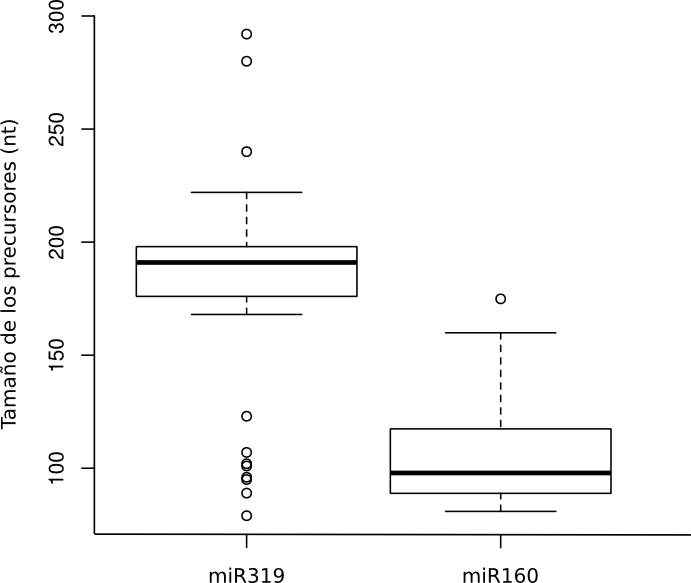
\includegraphics[width=.7\textwidth]{hairpin_distribution.png}
    \caption[Tamaño de precursores]{Tamaño de precursores. Se muestra el tamaño (nt) de dos familias de precursores en distintas especies.}
    \label{fig:hairpin_distribution}
\end{figure}

En particular, la biogénesis de los miARNs es un proceso clave porque determina la secuencia exacta de nucleótidos del ARN pequeño funcional.
Si bien en el caso de animales está claro cuáles elementos estructurales son reconocidos en los precursores durante su procesamiento, poco se sabía sobre el reconocimiento de los precursores de plantas por la maquinaria de procesamiento.

Muchos precursores en plantas tienen un tallo de $\sim$15 nt debajo del duplex miARN/miARN* seguido por un loop interno, que sirve como una señal estructural de reconocimiento por la maquinaria de procesamiento \citep{pmid17369351,pmid16751099,Mateos2010,pmid20015654}.
Sin embargo, este determinante de procesamiento no se encuentra en todos los precursores \citep{Mateos2010}.
Además, la biogénesis de los miARNs conservados evolutivamente como ser el miR319 y miR159 comienzan con un corte al lado del loop interno y continúa con 3 cortes adicionales en una dirección de burbuja a base hasta que finalmente el miARN es liberado \citep{Bologna2013,pmid19850910}.
Se ha demostrado que otros precursores de plantas liberan otros ARNs pequeños además del miARN \citep{pmid15314213,pmid20696037}, aunque los mecanismos de procesamiento subyacentes eran desconocidos.

\section{Resultados} 

\subsection{Procesamiento de precursores de miARNs en plantas}

En esta parte del proyecto de tesis y en el marco de una colaboración con el grupo del Dr. Blake Meyers (Delaware,USA), el cual se especializa en secuenciación y análisis de ARN pequeños, nos propusimos entender cómo se procesan los precursores de miARNs plantas. 
Colegas del laboratorio realizaron una estrategia para analizar sistemáticamente intermediarios de procesamiento de miARNs y caracterizar la biogénesis de la mayoría de los miARNs conservados presentes en \textit{A. thaliana} mediante técnicas de secuenciación de alto rendimiento, utilizando los equipos de última generación disponibles en Delaware (USA).
Esta técnica desarrollada en el laboratorio se conoce como sPARE \citep{Schapire2013} (del inglés Specific Parallel Amplification of RNA Ends).
Utilizando esta técnica encontramos que los miARNs son procesados por cuatro mecanismos, dependientes de la dirección secuencial de la maquinaria de procesamiento y del número de cortes requeridos para liberar el miARN.
La clasificación de los precursores, teniendo en cuenta los mecanismos de procesamiento, reveló determinantes estructurales específicos para cada grupo.
Se encontró que la complejidad de las vías de procesamiento de miARN se produce tanto en precursores jóvenes como en conservados y que los miembros de la misma familia pueden ser procesados de diferentes maneras.
Además hemos observado que diferentes determinantes estructurales compiten por la maquinaria de procesamiento y que miRNAs alternativos pueden ser generados a partir de un único precursor.
Los resultados ofrecen una explicación para la diversidad estructural de los genes de precursores de miARN en plantas y nuevas perspectivas hacia la comprensión de la biogénesis de los ARNs pequeños \citep{Bologna2013}.


\subsubsection{Análisis de datos y precursores detectados}
Mediante la cantidad de cortes detectados la técnica de sPARE permite definir si el mecanismo es base a loop o loop a base.
Esta técnica arroja una gran cantidad de datos producto de la secuenciación de alto rendimiento, por lo que se necesita de un enfoque bioinformático para la interpretación de los resultados.
Por la gran cantidad de precursores a estudiar y el número de bibliotecas se necesitó un análisis previo de los datos y una forma de presentarlos.
Para esto construimos e implementamos un pipeline bioinformático utilizando "in-house" scripts y datos disponibles de miRBASE para poder analizar los datos de las bibliotecas de deep-sequencing obtenidos a partir de la técnica de SPARE.

Un precursor fue considerado como detectado si más de tres lecturas corresponden a la secuencia de ese precursor.
De esta manera encontramos fragmentos de ARN que corresponden a 129 precursores, 71 de ellos de miARNs conservados y 58 de miARNs jóvenes (Figura \ref{fig:GR_fig1C}).
Mediante el análisis de los datos arrojados de la estrategia bioinformática pudimos definir la dirección de procesamiento de la mayoría de los precursores en \textit{A. thaliana}.
De los cuales 32 de ellos fueron definidos como procesados por un mecanismo de base a loop, ya que se encontraron los cortes en la parte proximal del duplex miARN/miARN* sin detectar cortes en la parte de arriba del duplex, como en el caso del miR168a, miR172b y el miR395b (Figura \ref{fig:GR_fig2A}).
Además encontramos 16 precursores de miARNs conservados con cortes detectados (>5\%) en el lado distal del miARN/miARN* los cuales fueron definidos como loop a base (Figura \ref{fig:GR_fig4A}).

\begin{figure}[htbp!] 
    \centering    
    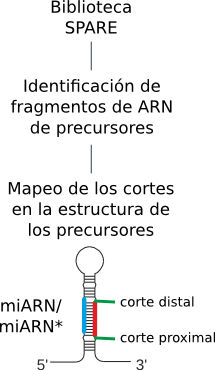
\includegraphics[width=.5\textwidth]{GR_fig1C.png}
    \caption[Esquema del procedimiento para analizar los datos de sPARE]{Esquema del procedimiento para analizar los datos de sPARE.}
    \label{fig:GR_fig1C}
\end{figure}

\begin{figure}[htbp!] 
    \centering    
    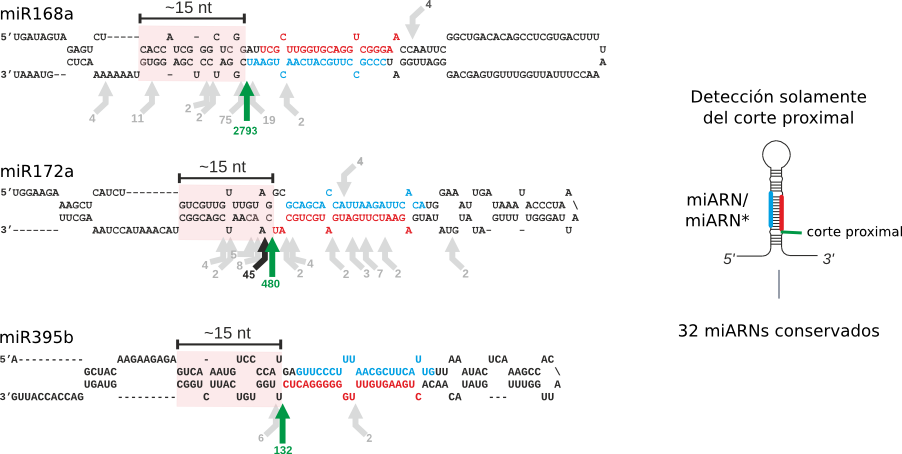
\includegraphics[width=1\textwidth]{GR_fig2A.png}
    \caption[Identificación y caracterización de precursores de miARNs procesados de base a loop]{Identificación y caracterización de precursores de miARNs procesados de base a loop.
            Esquema donde se muestra la estructura secundaria del miR168a, miR172b y miR395b.
            Las flechas indican la posición y número de lecturas de los cortes del precursor identificado.
            Flechas en verde muestra el corte más abundante, que también coincide con al corte proximal del miARN/miARN*.
            Flechas en negro muestran otros cortes con al menos 5\% de abundancia del número total de cortes, mientras que otros cortes minoritarios se muestran con una flecha gris.
            Con rosa se resalta el stem de 15nt debajo del corte proximal.
            El miARN se indica en color rojo y el miARN* en color azul.
            La imagen de la derecha muestra el patrón de corte típico detectado en la biblioteca de sPARE para estos precursores.}
    \label{fig:GR_fig2A}
\end{figure}


\begin{figure}[htbp!] 
    \centering    
    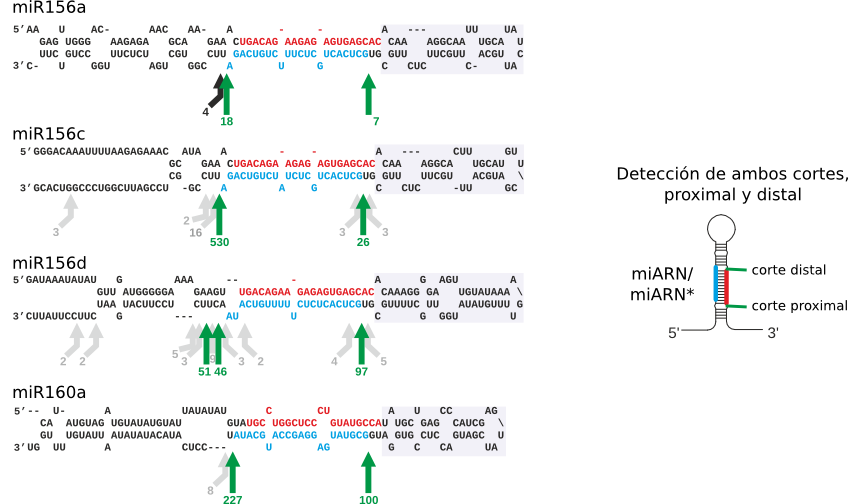
\includegraphics[width=1\textwidth]{GR_fig4A.png}
    \caption[Identificación y caracterización de precursores de miARNs procesados de loop a base]{Identificación y caracterización de precursores de miARNs procesados de loop a base. 
    Esquema donde se muestra la estructura secundaria del miR156a, miR156c, miR156d y miR160a.
    Las flechas indican la posición y número de lecturas de los cortes del precursor identificado.
    Flechas en verde muestra el corte más abundante, que también coincide con al corte proximal del miARN/miARN*.
    Flechas en negro muestran otros cortes con al menos 5\% de abundancia del número total de cortes, mientras que otros cortes minoritarios se muestran con una flecha gris.
    Con gris se resalta el stem de arriba del miR156 y miR160. El miARN se indica en color rojo y el miARN* en color azul.
    La imagen de la derecha muestra el patrón de corte típico detectado en la biblioteca de SPARE para estos precursores.
}
    \label{fig:GR_fig4A}
\end{figure}

\subsubsection{Estructura secundaria de los precursores}
Para ver si había diferencias estructurales para los precursores con diferentes mecanismos de procesamiento, determinamos la estructura secundaria de precursores detectados que se procesan en dirección base a loop (Figura \ref{fig:GR_fig2C}) y los que se procesan loop a base (Figura \ref{fig:GR_fig4C}).
Obtuvimos las estructuras secundarias para cada precursor.
Definimos a una coincidencia en cada posición con un 0, mientras que "bulges" y "mismatches" los consideramos como 1.
El lado proximal del duplex miARN/miARN* fue definido como la posición +1 y analizamos desde la posición -25 a la posición +40 (Figura \ref{fig:GR_fig2C} y \ref{fig:GR_fig4C}). 

\subsubsection{Procesamiento de base a loop}

Consideramos la estructura secundaria de 32 precursores analizados en esta parte del trabajo que se procesan de base a loop y todos ellos tienen un claro tallo inferior de 15 nt de largo (Figura \ref{fig:GR_fig2C}).
Además este tallo se pudo ver tanto para los precursores validados experimentalmente que se procesan de base a loop como para todos los precursores conservados (Figura \ref{fig:GR_fig2C} en violeta).
Pero pudimos observar que las bases inmediatamente debajo del duplex miARN/miARN* (posición -2 y -1) tienden a estar desapareadas (Figura \ref{fig:GR_fig2C}).
Además las posiciones -3 y -4 y las 3 últimas posiciones del stem inferior (-13,-14 y -15) están apareadas casi siempre (Figura \ref{fig:GR_fig2C}).
En general, nuestros resultados muestran que los precursores procesados en una dirección base a loop son más uniformes de lo que se pensaba previamente y que al menos algunos de los precursores no detectados como base a loop probablemente tengan otros determinantes específicos de ARN.

\subsubsection{Procesamiento de loop a base}
Estos precursores, que tienen un procesamiento loop a base, tienen un corte mayoritario que se puede detectar en nuestras bibliotecas.
Este corte es el esperado en la dirección de procesamiento de precursores con un mecanismo de loop a base.
Con la excepción de dos miARNs (miR396a y miR162b) estos precursores no tienen una estructura obvia debajo del duplex miARN/miARN* (Figura \ref{fig:GR_fig4C}).
Estos precursores tienen una región terminal estructurada (Figura \ref{fig:GR_fig4C}), que tiene un tamaño homogéneo de ~42nt que incluye un loop corto en contraste con la misma región en los precursores que se procesan de base a loop donde es más variable (Figura \ref{fig:GR_fig2C} y \ref{fig:GR_fig4C}). 

En esta segunda parte del proyecto de tesis presentamos un estrategia y realizamos un análisis sistemático para la identificación de la biogénesis de precursores de miARNs desde un punto de vista genómico.
De esta manera pudimos encontrar la dirección de procesamiento de la mayoría de los precursores de miARNs en \textit{A. thaliana}.

\begin{figure}[htbp!] 
    \centering    
    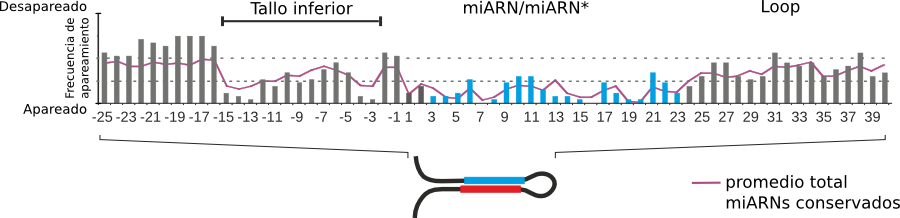
\includegraphics[width=1\textwidth]{GR_fig2C.png}
    \caption[Estructura secundaria de precursores de base a loop]{Estructura secundaria de precursores detectados que se procesan en dirección base a loop.
    Los matches en cada posición los consideramos como 0, mientras que "bulges" y "mismatches" fueron considerados como 1.
    La estructura secundaria considerando todos los miARNs conservados se indica con color violeta.
    }
    \label{fig:GR_fig2C}
\end{figure}

\begin{figure}[htbp!] 
    \centering    
    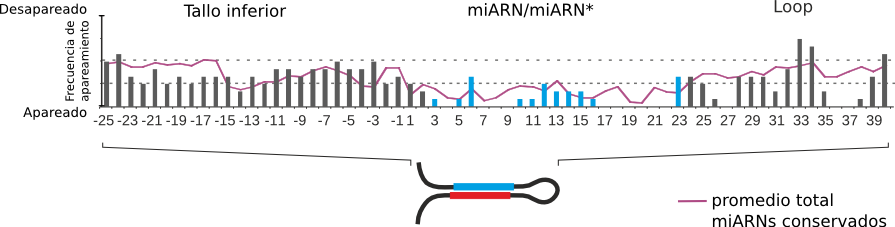
\includegraphics[width=1\textwidth]{GR_fig4C.png}
    \caption[Estructura secundaria de precursores de loop a base]{
    Estructura secundaria de precursores detectados que se procesan en dirección loop a base.
    Los matches en cada posición los consideramos como 0, mientras que "bulges" y "mismatches" fueron considerados como 1.}
    \label{fig:GR_fig4C}
\end{figure}


Estos resultados fueron publicado en la revista Genome Research \citep{Bologna2013}.
Em este mismo artículo se pudo demostrar que los precursores de miARNs en plantas, se pueden agrupar por cuatro mecanismos de procesamiento con distintas características (Figura \ref{fig:mecanismos}).

\begin{itemize}
    \item En los precursores con un mecanismo \textbf{corto de base a loop}, un loop interno seguido por un tallo inferior de $\sim$15nt especifica la posición del primer corte.
        Esta estructura se encuentra en la mayoría de familias de miARNs \citep{Mateos2010,pmid20015653,pmid20015654}.
        A pesar de que el tallo puede contener bulges, la transición de un loop interno (simple hebra) al tallo inferior es bastante marcada, y tres pares de bases apareadas generalmente definen el comienzo del tallo inferior del precursor \citep{Bologna2013}.
        El segundo corte procede a una distancia fija de $\sim$21 nt desde la posición del primer corte.
    \item En los precursores con un mecanismo \textbf{secuencial de base a loop} (ej: familia del miR169), el primer corte procede como en los cortos de base a loop, pero luego son necesario dos cortes más para liberar el miARN, generando en el proceso niveles bajos de RNA pequeños adicionales \citep{Bologna2013}.
    \item En los precursores con un mecanismo \textbf{cortos de loop a base} (ej: familia del miR156 y miR160), el procesamiento es guiado por un tallo superior, y son necesarios dos cortes para liberar el miARN maduro.
        La región terminal de estos precursores tienen una largo conservado de $\sim$42 donde incluye un loop pequeño \citep{Bologna2013}.
    \item En los precursores con un mecanismo \textbf{secuencial de loop a base} (ej: familia del miR319 y miR159), cuatro cortes secuenciales por DCL1 son los encargados de procesar los precursores de miARNs.
        En general muestran un tallo largo superior, del cual otros ARNs pequeños son generados \citep{pmid19850910,Bologna2009,Bologna2013}
\end{itemize}

\begin{figure}[htbp!] 
    \centering    
    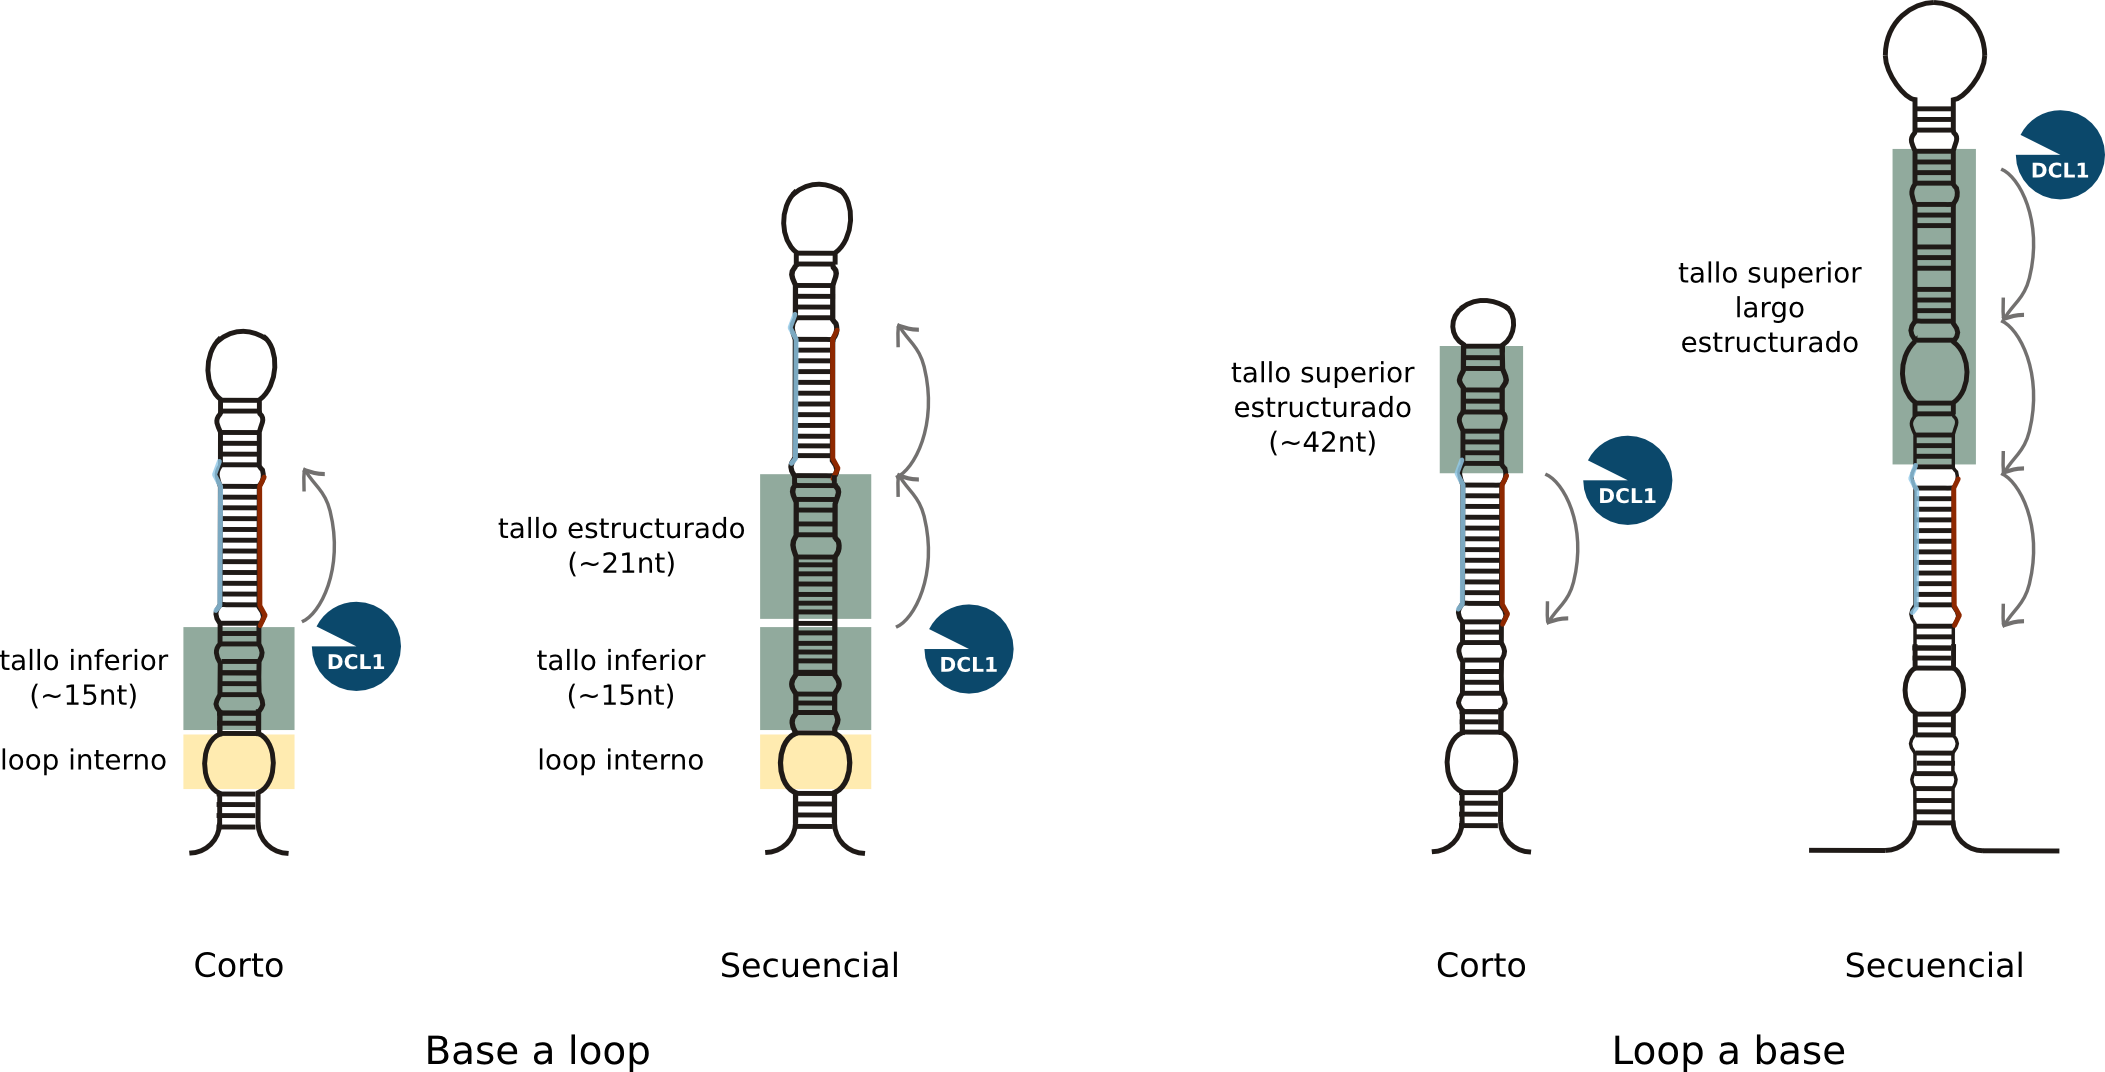
\includegraphics[width=1\textwidth]{mecanismos.png}
    \caption[Mecanismos de procesamiento]{Distintos mecanismos de procesamientos de miARNs en plantas}
    \label{fig:mecanismos}
\end{figure}

\subsection{Enfoque bioinformático para el estudio de la evolución y biogénesis de miARNs en plantas}

Que los precursores de miARNs en plantas sean procesados de diferentes maneras \citep{Bologna2013}, nos llevó a especular que su patrón de evolución también puede ser diferente y podrían estar vinculados a su mecanismo de procesamiento.
Es por esto que elaboramos una estrategia bioinformática para caracterizar la relación entre la evolución de los precursores de miARNs en plantas y los mecanismos de procesamiento determinados previamente.

\subsubsection{Estrategia}

La metodología utilizada se detalla en la sección \ref{ref_evolution} y primero la utilizamos para estudiar precursores de miARNs conservados en dicotiledóneas. 
La misma consta de los siguientes pasos:

\begin{itemize}
    \item Búsqueda de ortólogos para cada miembro de cada familia de Arabidopsis de  precursores de miARNs conservados en plantas
    \item Extensión de las secuencias
    \item Alineamiento de secuencia primaria
    \item Alineamiento de secuencia teniendo en cuenta estructura secundaria
    \item Búsqueda de motivos conservados
    \item Representación gráfica de los precursores
\end{itemize}

\subsubsection{Búsqueda de ortólogos de precursores de miARNs}

Las secuencias de los precursores de miARNs en miRBASE rara vez son validadas experimentalmente, de hecho muchas de ellas son el resultado de predicciones computacionales de estructuras en forma de tallo y burbuja que incluye el miARN maduro, pero que no se extiende muchas bases más allá de el mismo \cite{Kozomara2014}.
Esto lleva a anotaciones erróneas de los precursores de miARNs.
Además para cada miembro de cada familia de \textit{A. thaliana} no es trivial asignarle un ortólogo en otra especie teniendo en cuenta la anotación de miRBASE.

Por esto, primero realizamos una búsqueda de ortólogos para cada miembro de cada familia de \textit{A. thaliana} y empezamos nuestro análisis con una definición arbitraria de los precursores de plantas incluyendo 150 nt fuera del par miARN/miARN*.
Para la búsqueda de ortólogos, extensión de la secuencia y el posterior análisis de los precursores, utilizamos datos genómicos de plantas extraídos de Phytozome. 

Para la mayoría de los miembros de cada familia de precursores pudimos detectar ortólogos en otras especies. 
Teniendo en cuenta las 30 dicotiledóneas utilizadas en este estudio, en promedio, se encontraron ortólogos para cerca de 20 especies para cada precursor de miARN de \textit{A. thaliana} (Figura \ref{fig:dicots_species}).

\begin{figure}[htbp!] 
    \centering    
    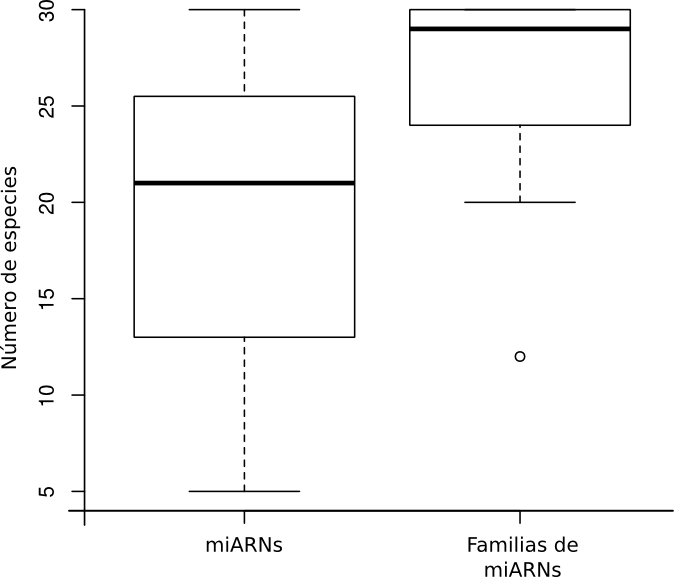
\includegraphics[width=.5\textwidth]{dicots_species.png}
    \caption[Especies detectadas]{Cantidad de especies detectadas.
    Esta figura muestra la distribución de la cantidad de especies donde se encuentran ortólogos de precursores de miARNs.
    A la izquierda se muestra la distribución de especies por miembro de familias de precursores de miARNs donde se detecta el ortólogo de \textit{A. thaliana}.
    A la derecha se agruparon todos los miembros de una misma familia y se muestra la distribución de la cantidad de especies donde se detecta un ortólogo de \textit{A. thaliana}}
    \label{fig:dicots_species}
\end{figure}

Algunos familias de miARNs se han diversificado durante la evolución, donde en algunas especies un miARN puede encontrarse como un único gen y en otras especie el mismo miARN puede encontrarse en múltiples miembros.
Por ejemplo, el miR396 en Arabidopsis está constituido por dos miembros, miR396a y miR396b mientras que en en el caso de arroz existen 8 miembros, nombrados del miR396a al miR396h.
Por esto, agrupamos a los miembros por familias y vimos la distribución de la cantidad de especies donde se detecta un ortólogo de los precursores de miARNs pertenecientes a \textit{A. thaliana} y en este caso vimos un alto número de especies detectadas para la mayoría de las familias de miARNs (Figura \ref{fig:dicots_species}).

\subsection{Alineamiento de los precursores en base a su secuencia primaria}

Comenzamos con los alineamientos múltiple de cada miembro de las familias de precursores de miARNs conservadas en dicotiledóneas.
Primero, realizamos el alineamiento en base a su secuencia primaria utilizando la herramienta T-Coffee \citep{pmid10964570}.
En la Figura \ref{fig:miR172a_tcoffee} se muestra el alineamiento del precursor del miR172a en distintas especies coloreado en base a la conservación evolutiva de la secuencia primaria.
Se puede observar que el miR172a maduro y el miR172a* están muy conservados en las distintas especies, pero además se puede ver una cola de conservación que podría corresponder al tallo inferior del precusor (Figura \ref{fig:miR172a_tcoffee}).

\begin{landscape}
    \begin{figure}[htbp!] 
        \centering    
        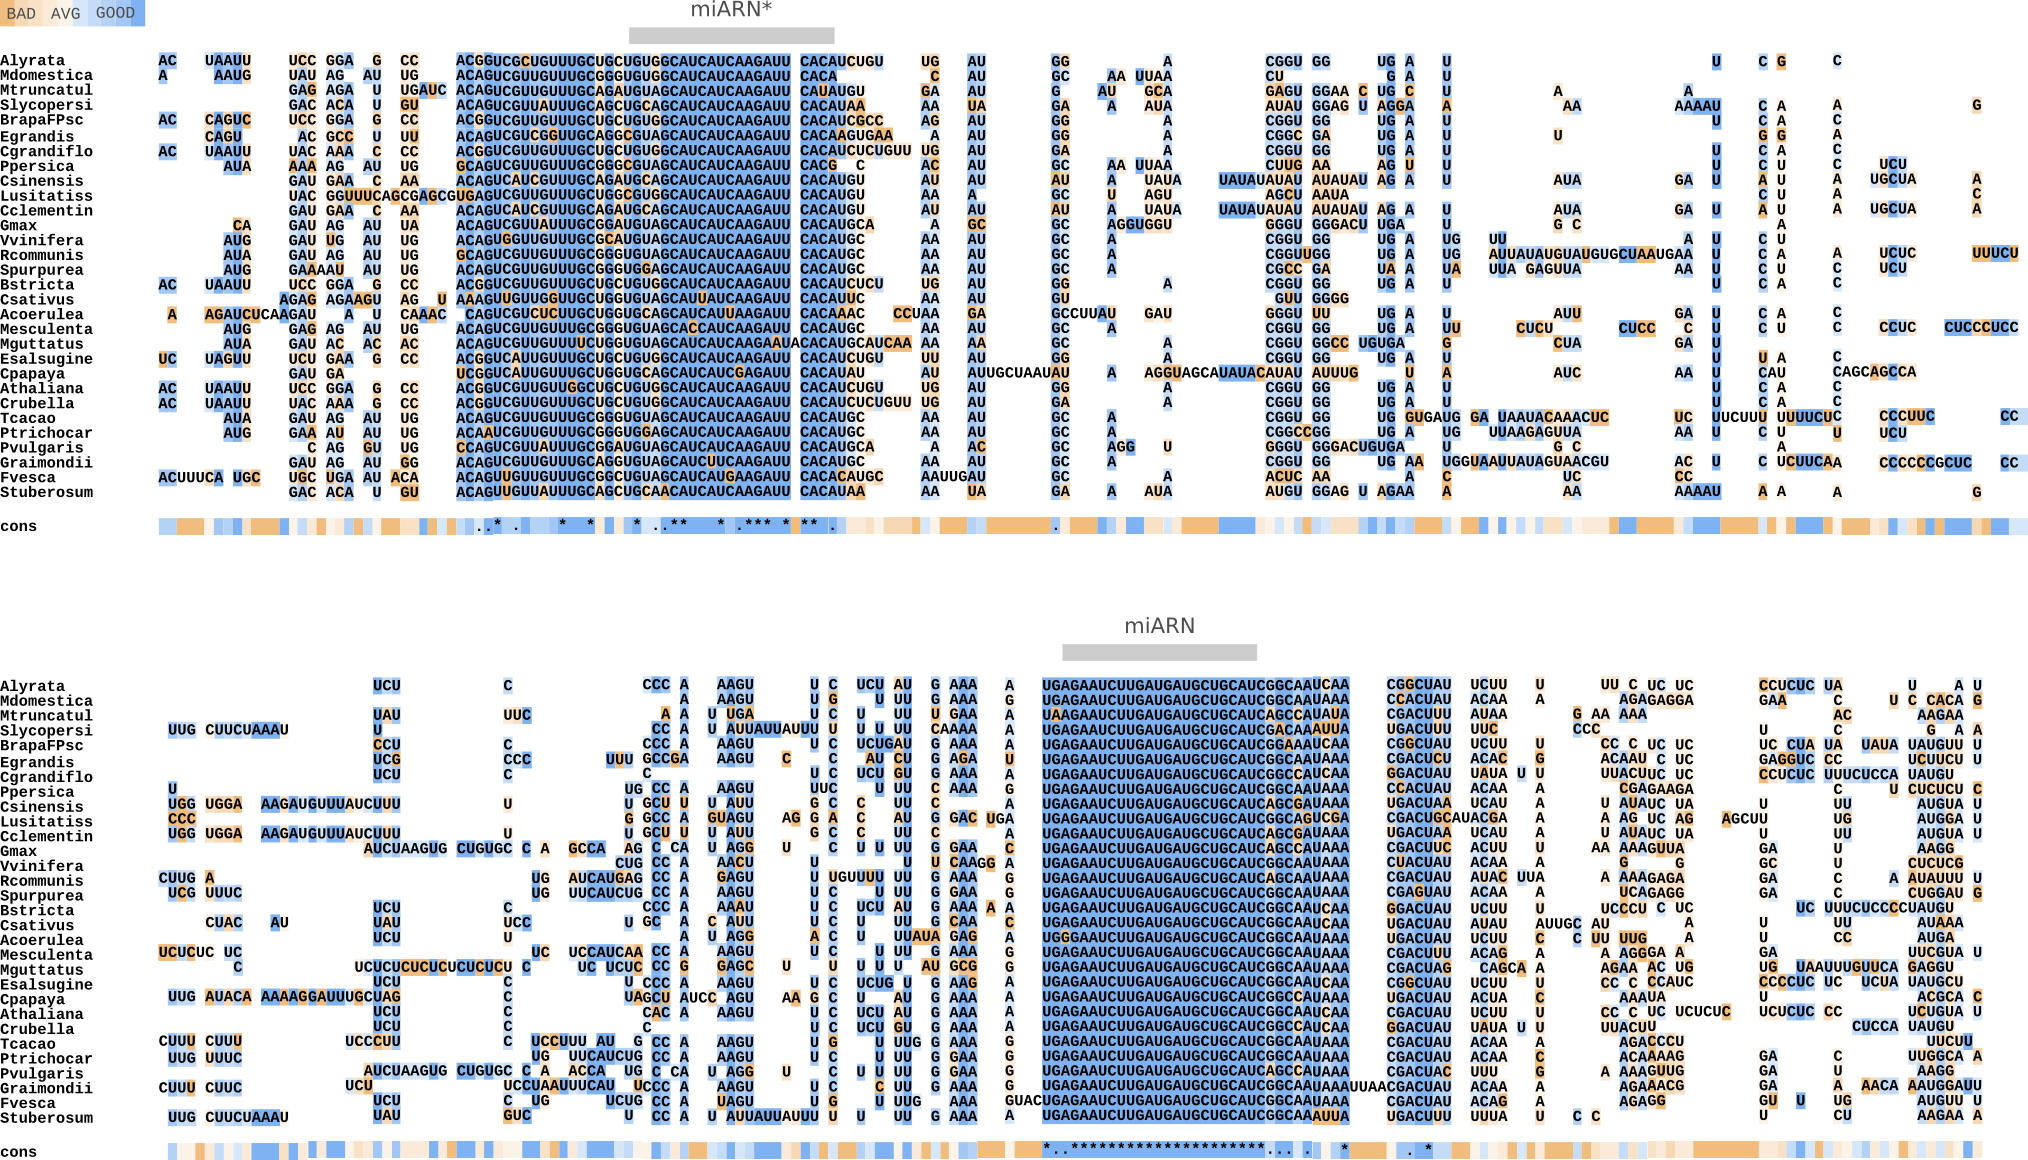
\includegraphics[width=1.4\textwidth]{miR172a_tcoffee.png}
        \caption[Alineamiento del precursor del miR172a.]{Alineamiento del precursor del miR172a. 
        Se muestra el alineamiento del precursor del miR172a en distintas especies. 
        En colores se muestra la conservación de la secuencia primaria, donde azul más oscuro denota mayor conservación y naranja menor conservación.
        Se muestran $\sim$60 bases por debajo del dúplex miARN/miARN* y los alineamientos están separados en dos líneas para una mejor representación.}
         \label{fig:miR172a_tcoffee}
    \end{figure}
\end{landscape}

Para poder corroborar esto y obtener información adicional sobre la conservación de los precursores, realizamos la predicción de estructura secundaria utilizando la herramienta RNAfold \citep{pmid22115189} (Figura \ref{fig:miR172a_rnafold}).
Además realizamos nuevamente los alineamientos pero considerando la estructura secundaria de los precursores, utilizando la herramienta R-Coffee \citep{pmid18292307}.

En la Figura \ref{fig:miR172a_rnafold} se puede observar que existe un patrón que comparten los precursores en la región debajo del miARN/miARN*.
No es simple reconocer patrones similares mirando los precursores de esta manera.
Además la cantidad de precursores estudiados en esta parte del trabajo de Tesis dificulta aún más este tipo de análisis.

\begin{landscape}
    \begin{figure}[htbp!] 
        \centering    
        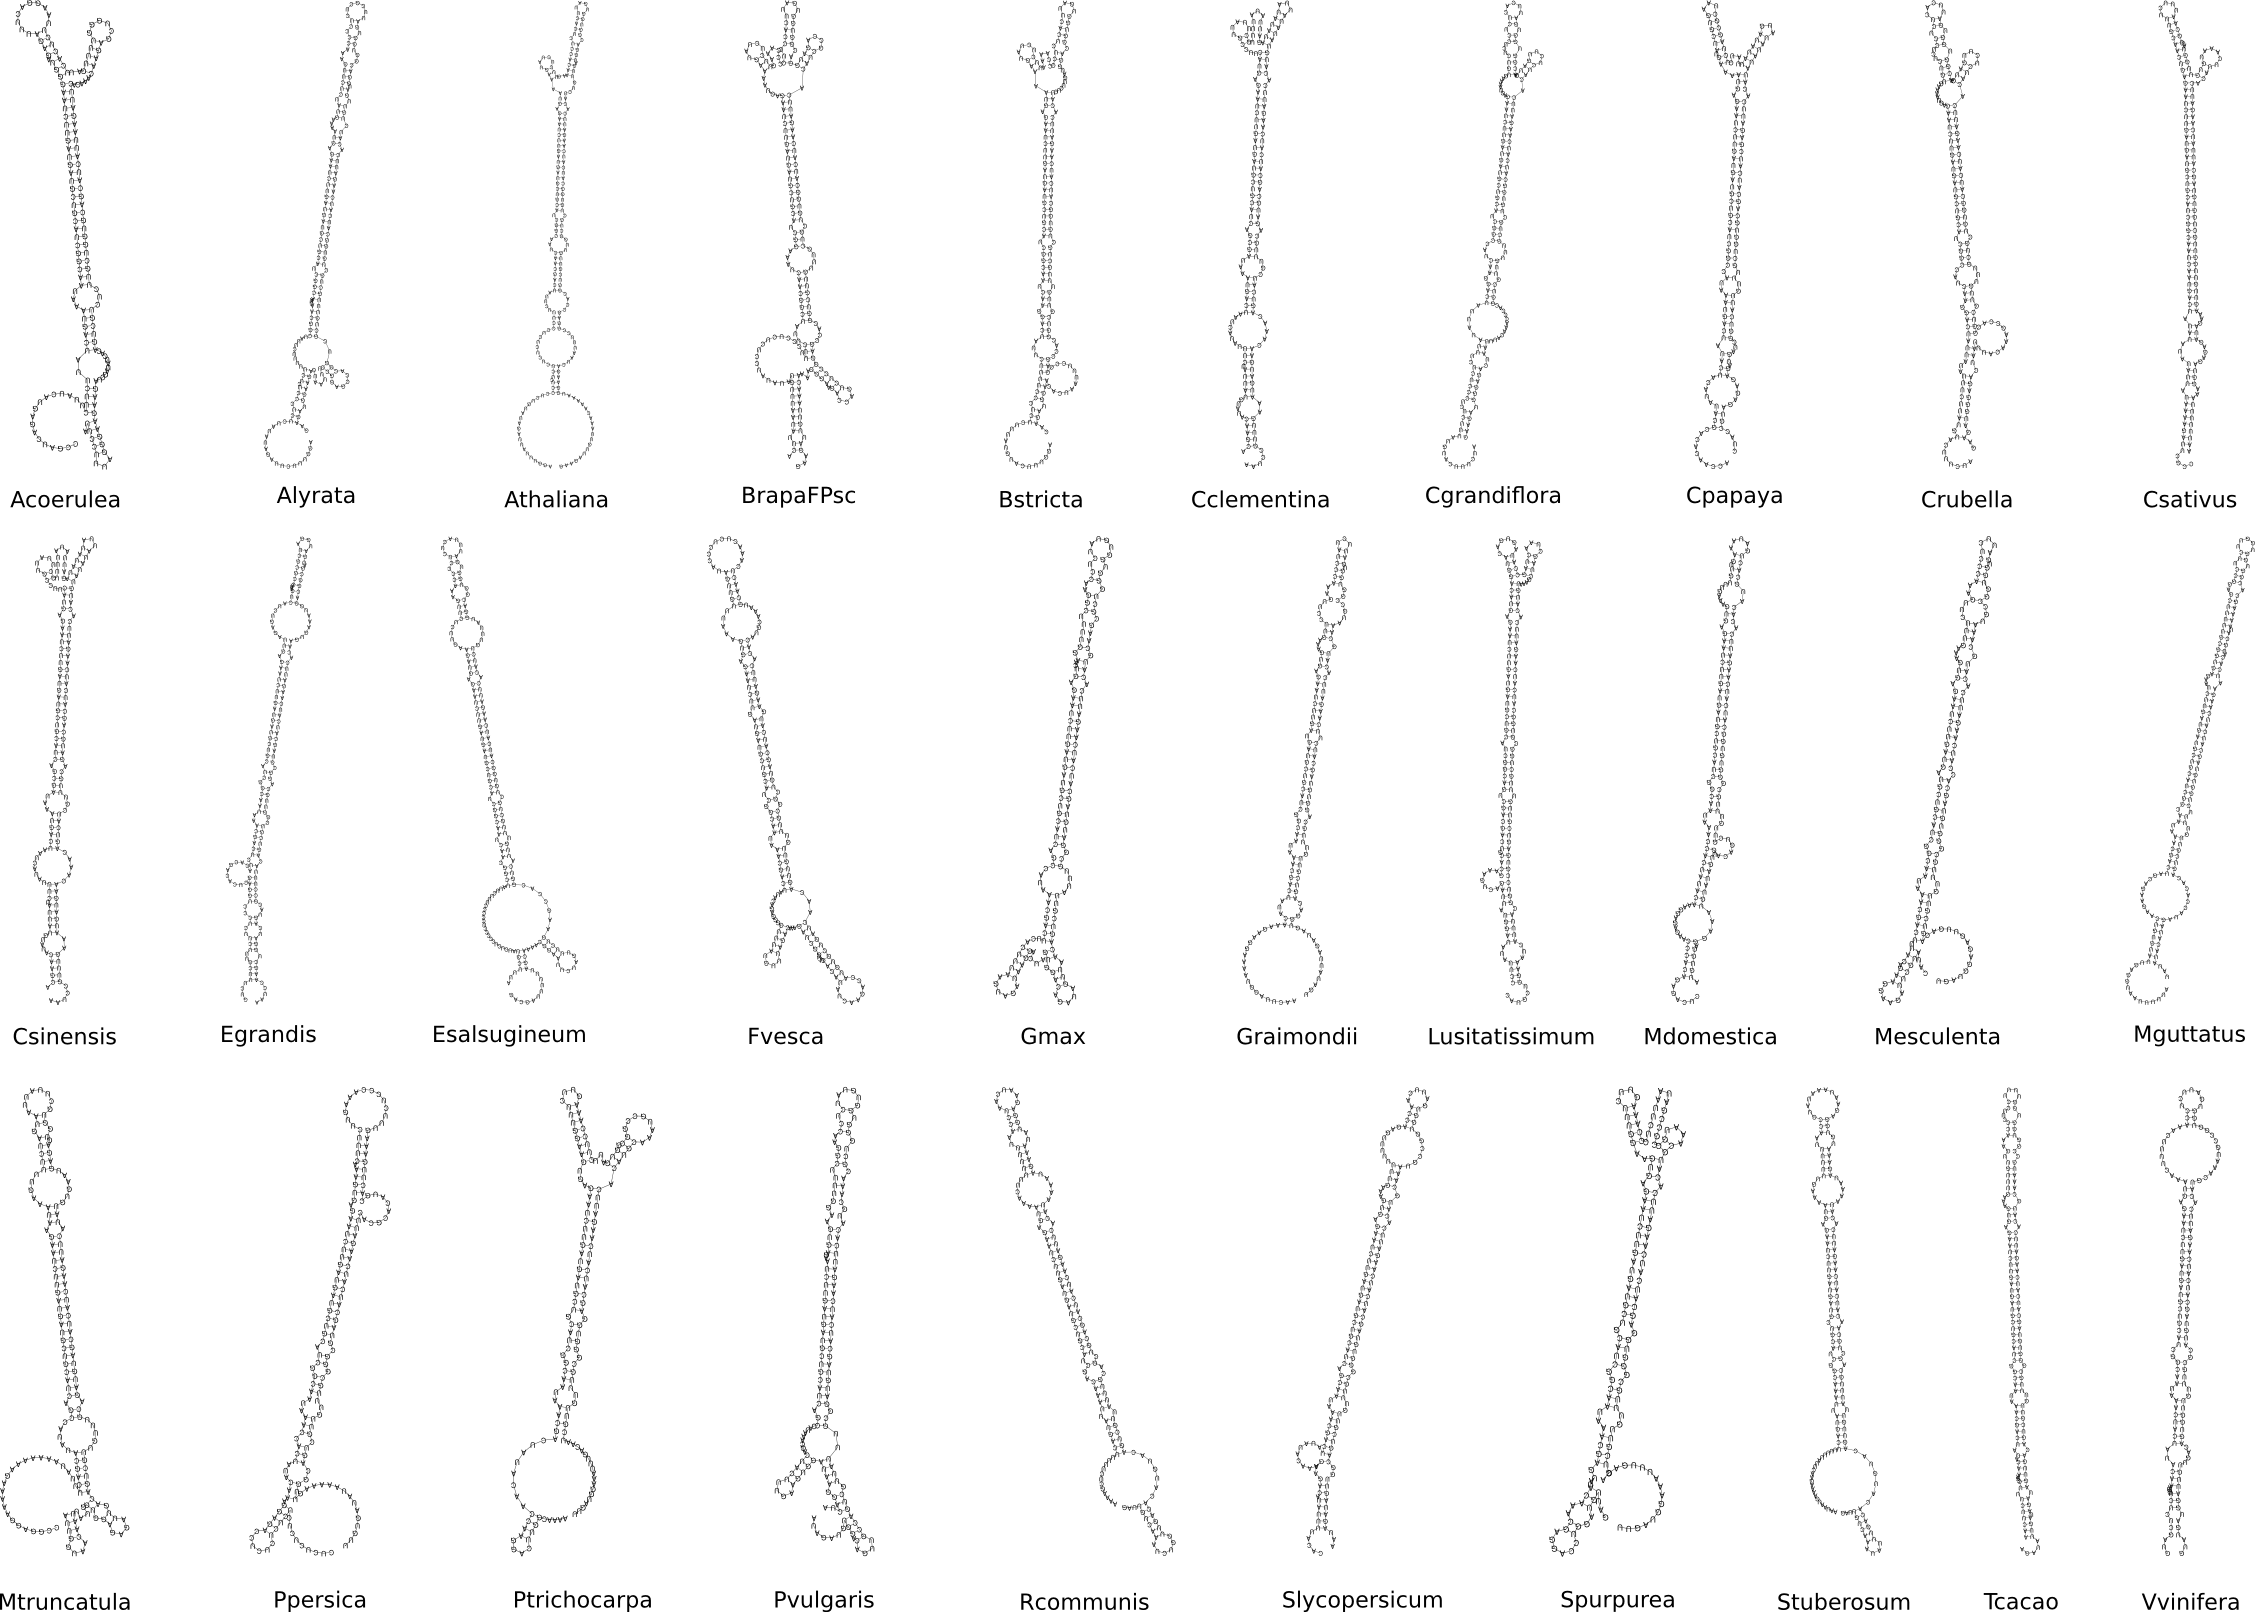
\includegraphics[width=1.4\textwidth]{miR172a_rnafold.png}
        \caption[Estructura secundaria del miR172a en distintas especies]{
        Estructura secundaria del miR172a en distintas especies.
        Se muestra la estructura secundaria de los precursores del miR172a en distintas especies, calculados con la herramienta RNAfold.
        }
        \label{fig:miR172a_rnafold}
    \end{figure}
\end{landscape}

Para poder reconocer fácilmente la región conservada dentro del precursor y poder analizar más en detalle estos patrones de conservación, decidimos agrupar toda esta información
 generada a partir de los alineamientos de secuencia primaria y estructura secundaria en un gráfico circular como se muestra en la figura \ref{fig:miR172a_circos}.
Estos gráficos se hicieron utilizando el paquete Circos \citep{pmid19541911}.
 
En dicha figura se muestra el Circos del miR172a a modo de ejemplo.
Para representar el precursor, se tomaron 60 nt por debajo del dúplex miARN/miARN*.
En el anillo exterior se representa en colores el grado de conservación de la secuencia consenso a partir de los alineamientos en base a su secuencia primaria.
Además se muestran las bases del precursor de \textit {A. thaliana}.
Luego en el anillo interior se representa, mediante un histograma, la frecuencia de bases apareadas y desapareadas para cada posición del precursor en las distintas especies.
Con líneas de distinto espesor se muestra la interacción de las bases del precursor considerando la estructura secundaria. 
Fuera del anillo exterior se marca la secuencia del miARN y miARN*.

Realizamos los Circos para visualizar de manera simple los precursores de miARNs en distintas especies de plantas.
Y los utilizamos para caracterizar la relación entre los patrones de conservación y los mecanismos de procesamiento determinados previamente.


\begin{figure}[htbp!] 
    \centering    
    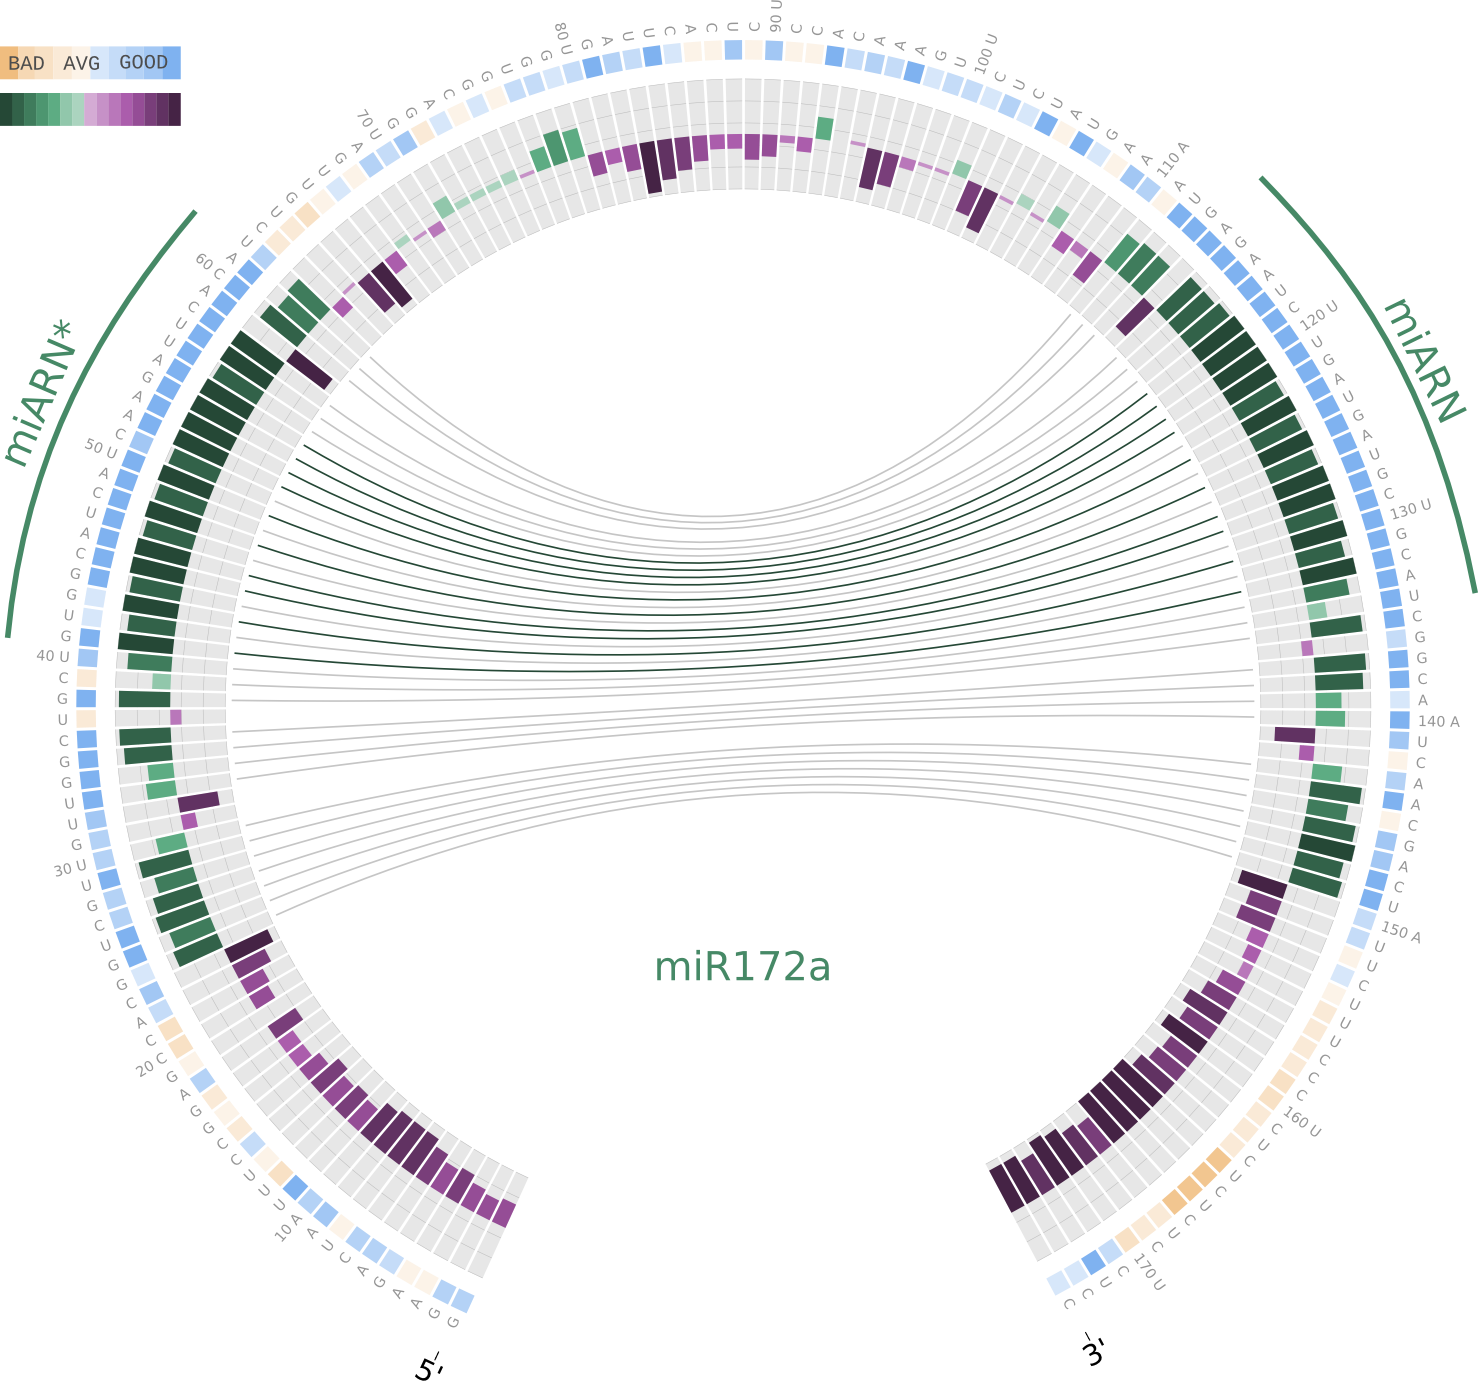
\includegraphics[width=1\textwidth]{miR172a_circos.png}
    \caption[Circos del miR172a]{Circos del miR172a.
En el anillo exterior se representa en colores el grado de conservación de la secuencia consenso a partir de los alineamientos en base a su secuencia primaria.
Además se muestran las bases del precursor de \textit {A. thaliana}.
Luego en el anillo interior se representa, mediante un histograma, la frecuencia de bases apareadas y desapareadas para cada posición del precursor en las distintas especies.
Con líneas de distinto espesor se muestra la interacción de las bases del precursor considerando la estructura secundaria. 
Fuera del anillo exterior se marca la secuencia del miARN y miARN*.
   }
     \label{fig:miR172a_circos}
\end{figure}

Por último, para cada precursor en distintas especies, realizamos una búsqueda de motivos conservados con la herramienta MEME \citep{pmid22115189} (Figura \ref{fig:miR172_meme}).
Hicimos esto para poder ver de manera visual cuáles eran los patrones comunes entre las distintas especies y donde se localizaban dentro del precursor.
Esta búsqueda de motivos la hicimos de diferentes maneras, la primera permitiendo encontrar hasta 2 motivos conservados en los precursores de distintas especies.


\begin{landscape}
    \begin{figure}[htbp!] 
        \centering    
        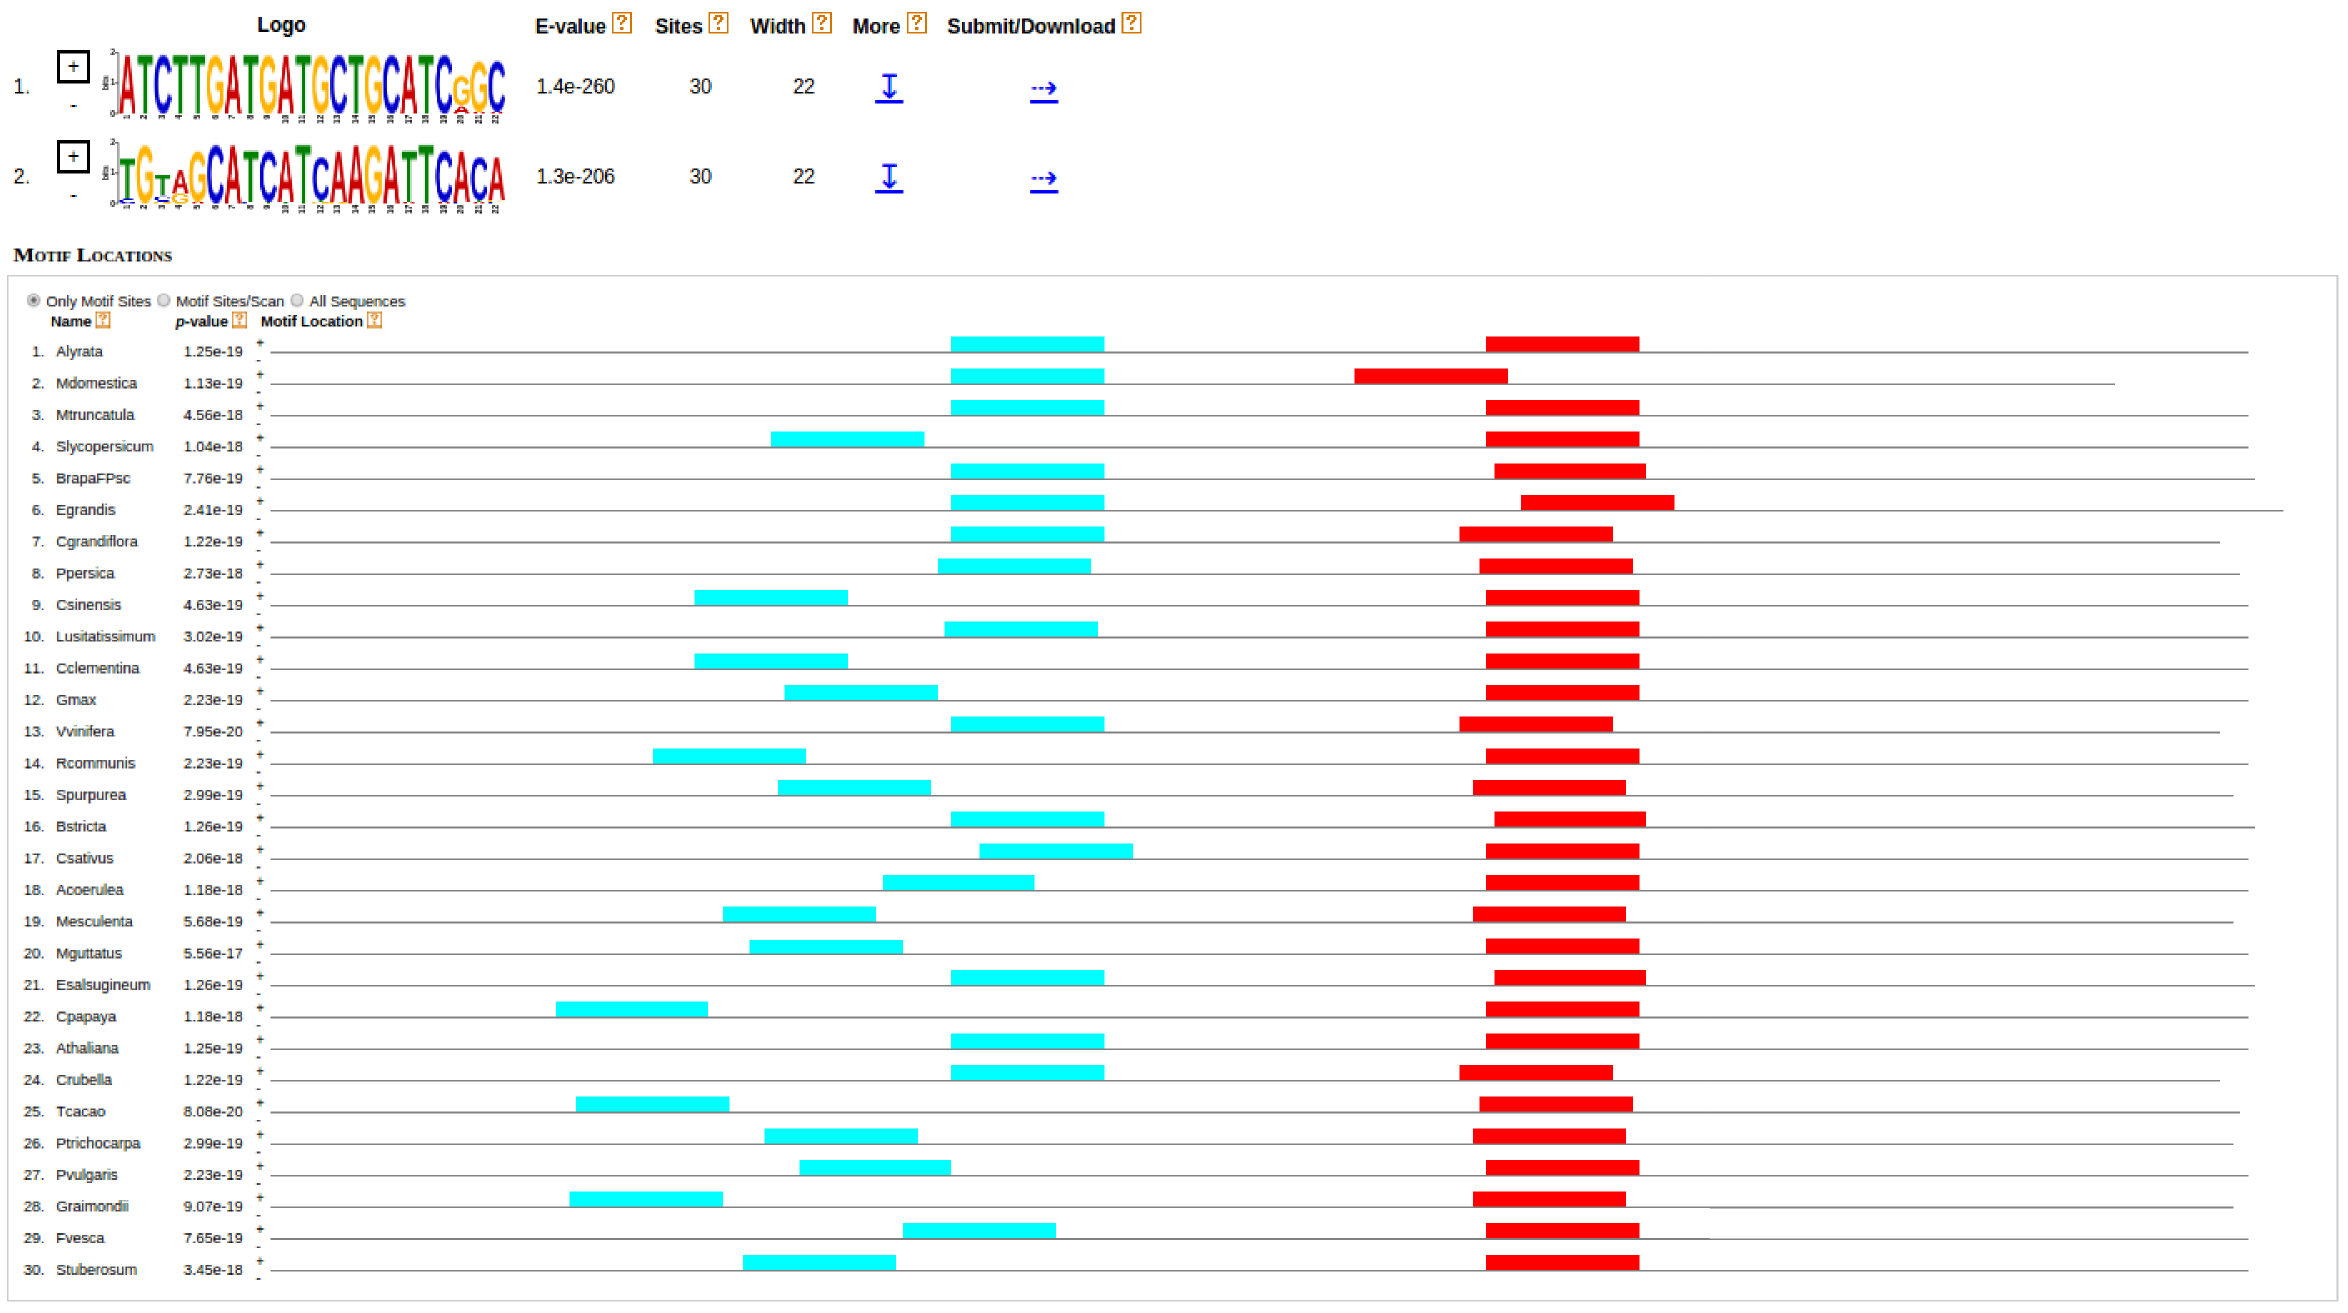
\includegraphics[width=1.4\textwidth]{miR172_meme.png}
        \caption[MEME del miR172a]{
			\textbf{MEME del miR172a.}
        Se muestra el MEME donde se pueden observar los motivos conservados dentro de los precursores del miR172a en distintas especies.
        En color rojo el primer motivo conservado comprende parte del miR172 (logo 1).
        El segundo motivo más conservado comprende parte del miR172* (logo 2).
        }
        \label{fig:miR172_meme}
    \end{figure}
\end{landscape}

\subsection{Mecanismo de base a loop cortos}

En los precursores con un mecanismo corto de base a loop, un loop interno seguido por un tallo inferior de $\sim$15nt especifica la posición del primer corte.
A pesar de que el tallo puede contener bulges, la transición de un loop interno (simple hebra) al tallo inferior es bastante marcada, y tres pares de bases apareadas generalmente definen el comienzo del tallo inferior del precursor \citep{Mateos2010,Bologna2013}.
El segundo corte procede a una distancia fija de $\sim$21 nt desde la posición del primer corte.

Para la mayoría de los precursores procesados con este mecanismo pudimos observar el mismo patrón de conservación de estructura primaria y similares patrones de estructura secundaria (Figura \ref{fig:miR172a_circos} y \ref{fig:miR390a_circos}). 
La región con mayor conservación conincide con el duplex miARN/miARN* pero además se puede ver una región  conservada por debajo del dúplex, que coincide con el tallo inferior.

Otra ventaja de esta forma de representar a los precursores y su conservación es que visualmente se puede reconocer facilmente posiciones "mismatches" conservados. 
Por ejemplo en el Circos del miR172, se puede observar un mismatch en la primer posición del miARN con la posición 19 del miARN*.
Esta interacción es A-A y se mantiene sin variaciones en todas las especies (Figura \ref{fig:miR172a_circos}).
Esto podría ser interesante estudiarlo en detalle donde se podría generar un precursor mutante donde esas bases en particular estén apareadas y luego ver si esto afecto o no el procesamiento del precursor.  

Además notamos que este patrón de conservación se puede observar independientemente si el miARN maduro está en la hebra 5' (Figura \ref{fig:miR172a_circos} ) o si está en la hebra 3' (Figura \ref{fig:miR390a_circos}).
A diferencia de los precursores que tienen un mecanismo de loop a base, donde el tallo superior es fundamental para el su procesamiento, los precursores que se procesan cortos de base a loop no tienen el tallo superior conservado.
Y mediante la búsqueda de motivos conservados, pudimos observar que el tamaño del tallo superior y del loop es muy variado en un mismo precursor en distintas especies, donde los mismos puede ir desde los 40nt hasta 115nt (Figura \ref{fig:miR172_meme}).


\begin{figure}[htbp!] 
    \centering    
    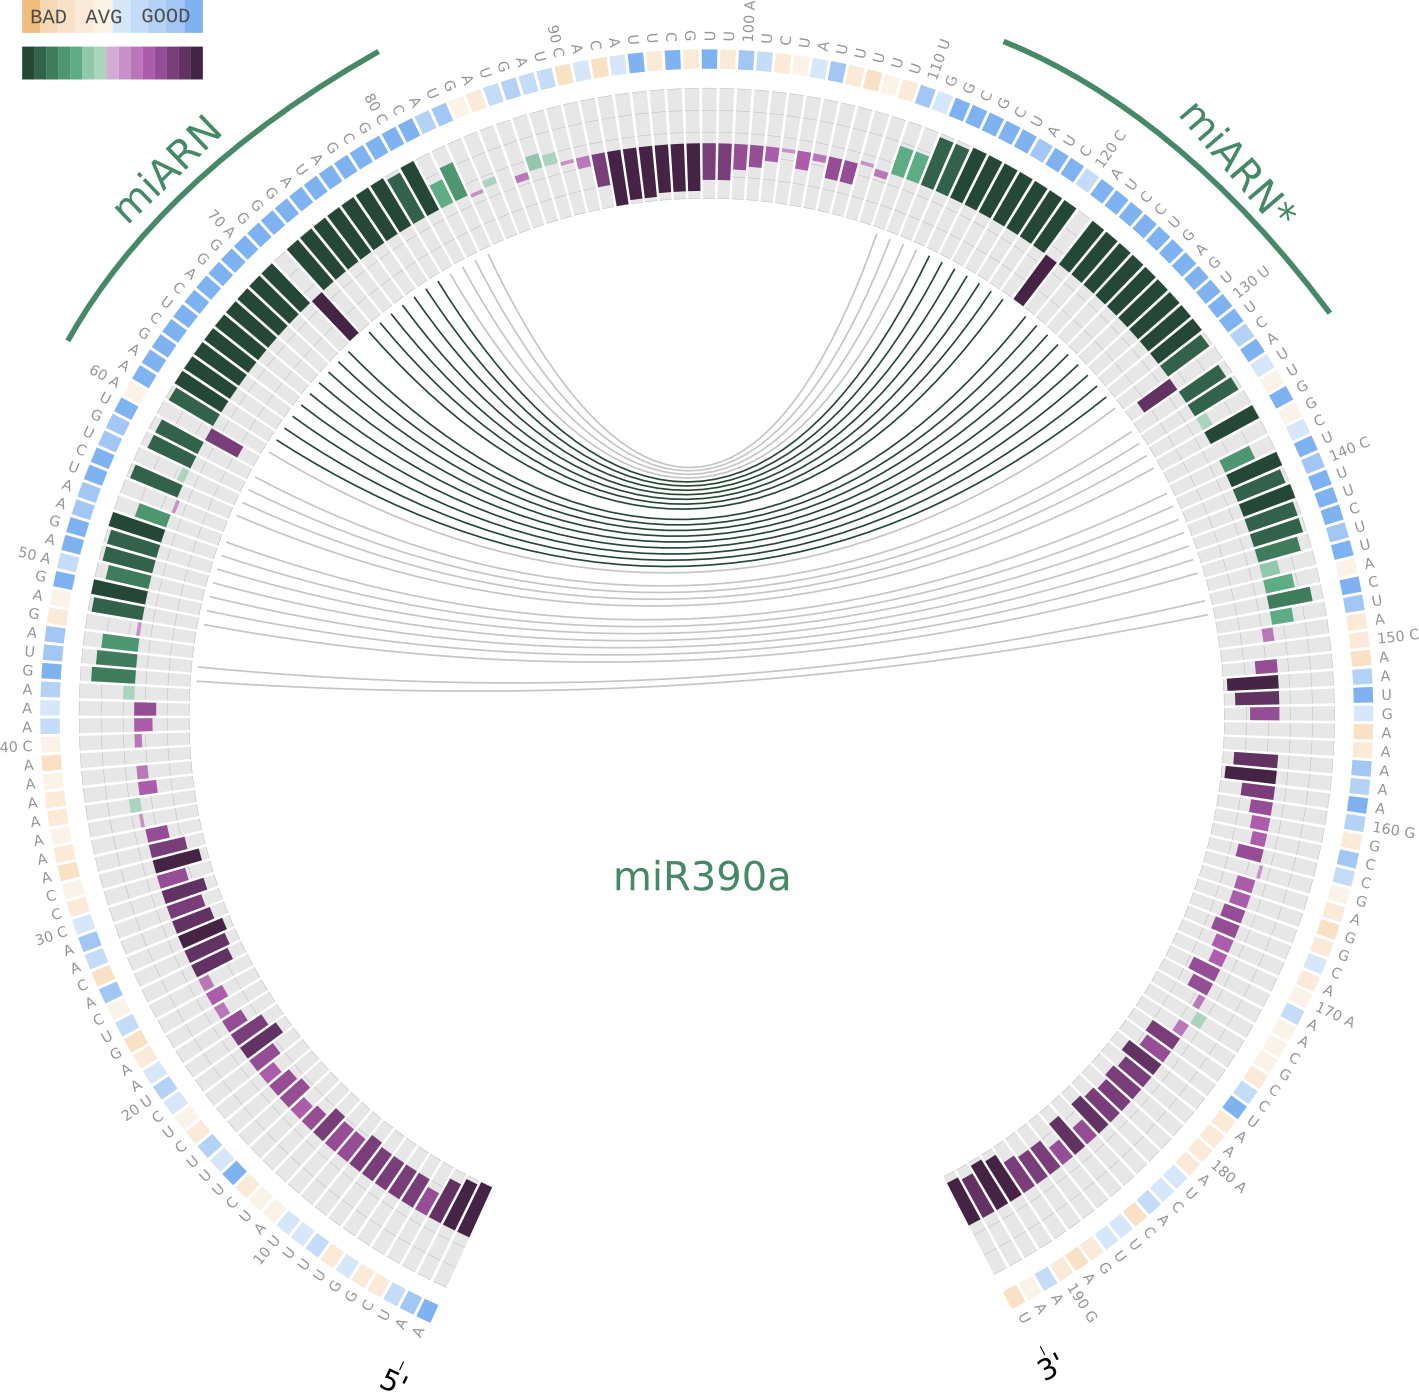
\includegraphics[width=1\textwidth]{miR390a_circos.png}
    \caption[Circos del miR172a]{Circos del miR390a.}
     \label{fig:miR390a_circos}
\end{figure}

\subsection{Mecanismo de base a loop secuenciales}

En estos precursores, con un mecanismo secuencial de base a loop, el primer corte procede como en los cortos de base a loop, pero luego son necesario dos cortes más para liberar el miARN, generando en el proceso niveles bajos de RNA pequeños adicionales \citep{Bologna2013}.
Este es el caso de algunos miembros de la  familias del miR169, que tiene en total 14 miembros siendo la familia más grande de \textit{A. thaliana}.
Un estudio en detalle de los precursores del miR169b/d/e/f/g mostró que los sitios de cortes del precursor estaban localizados 21 nt por debajo del lado proximal del dúplex miARN/miARN*.
Esta es la distancia esperada entre dos cortes de DCL1, sugeriendo que estos precursores eran procesados por más de dos cortes de la encima \citep{Bologna2013}.

La familia del miR394 también es procesada de la misma manera y comparten similares patrones de estructura secundaria, donde se ve el tallo inferior largo bien estructurado (Figura \ref{fig:seqBTL_circos}).
Si observamos el patrón de conservación de secuencia primaria podemos ver que la región del dúplex miARN/miARN está muy conservada, pero además podemos observar que debajo del dúplex existe otra región conservada que coincide con el tallo inferior largo que presentan estos precursores (Figura \ref{fig:seqBTL_circos}).


\begin{landscape}
	\begin{figure}
	\centering
	\begin{subfigure}{.75\textwidth}
	  \centering
	  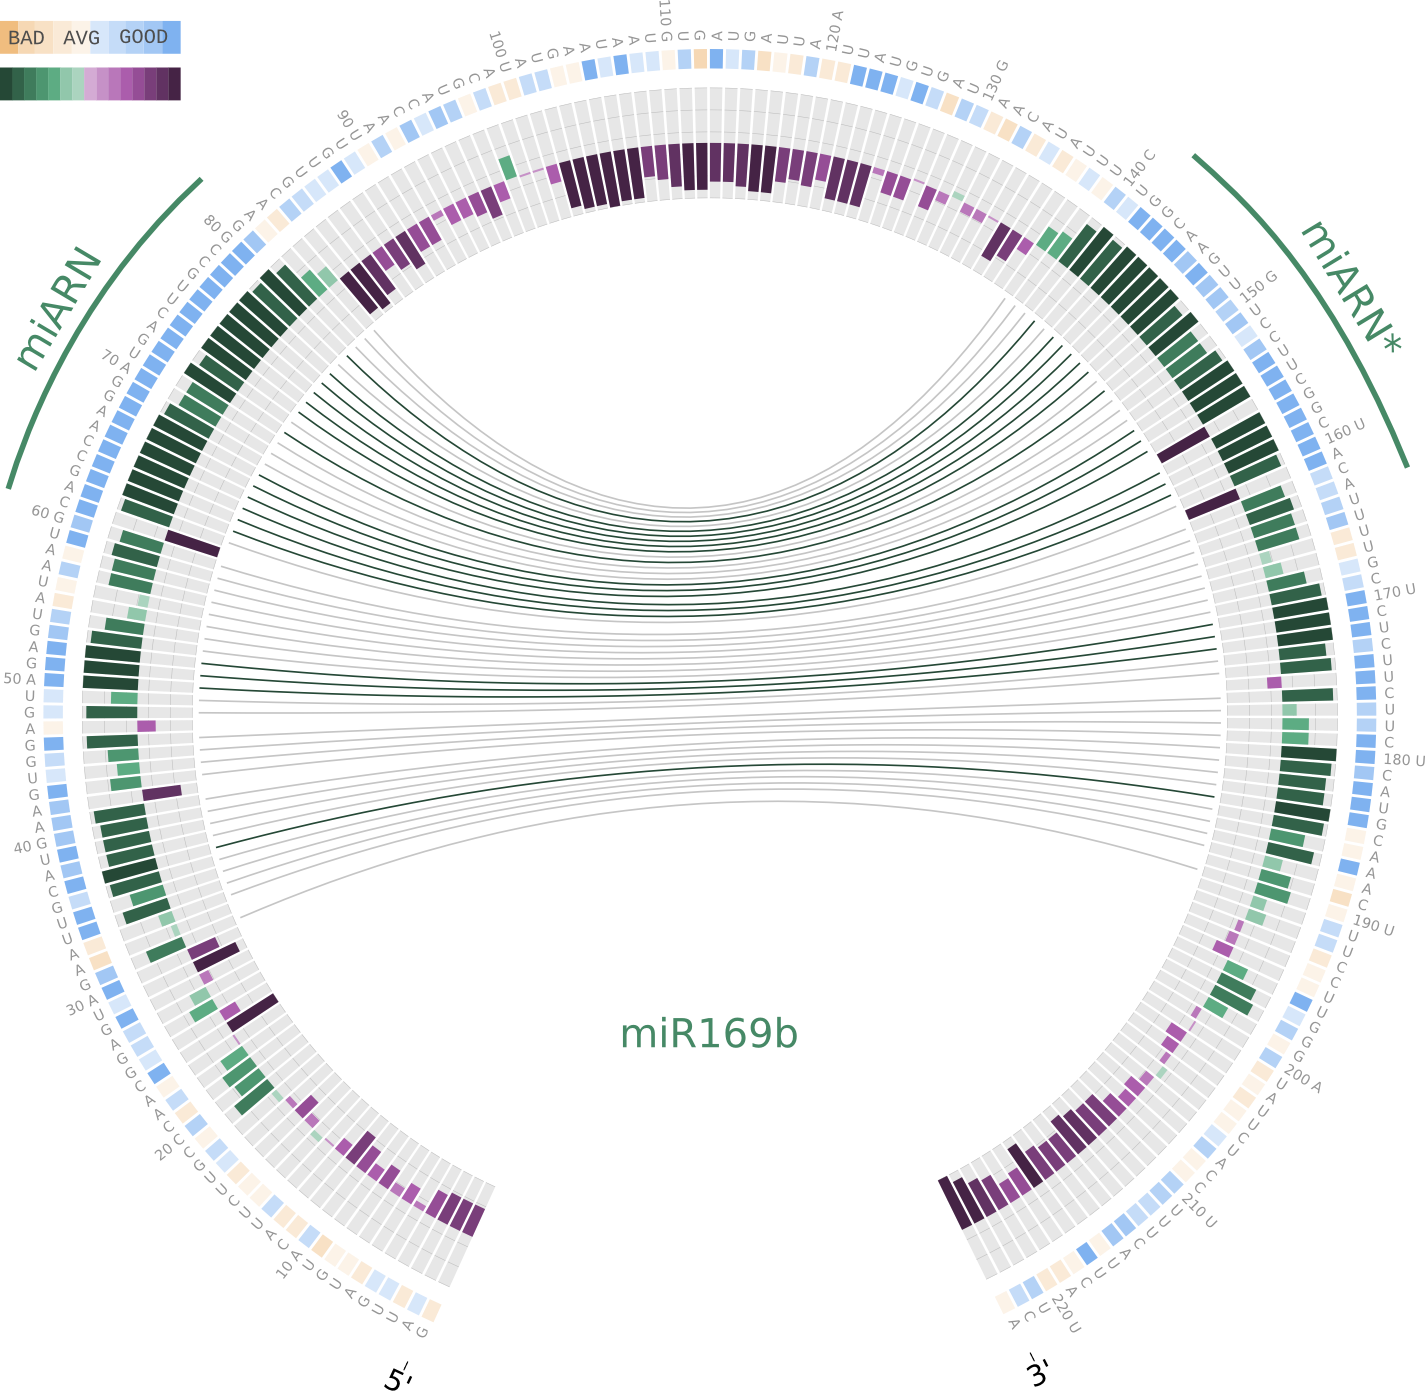
\includegraphics[width=.9\linewidth]{miR169b_circos.png}
	  \caption{Precursor del miR169b}
	  \label{subfig:miR169b_circos}
	\end{subfigure}%
	\begin{subfigure}{.75\textwidth}
	  \centering
	  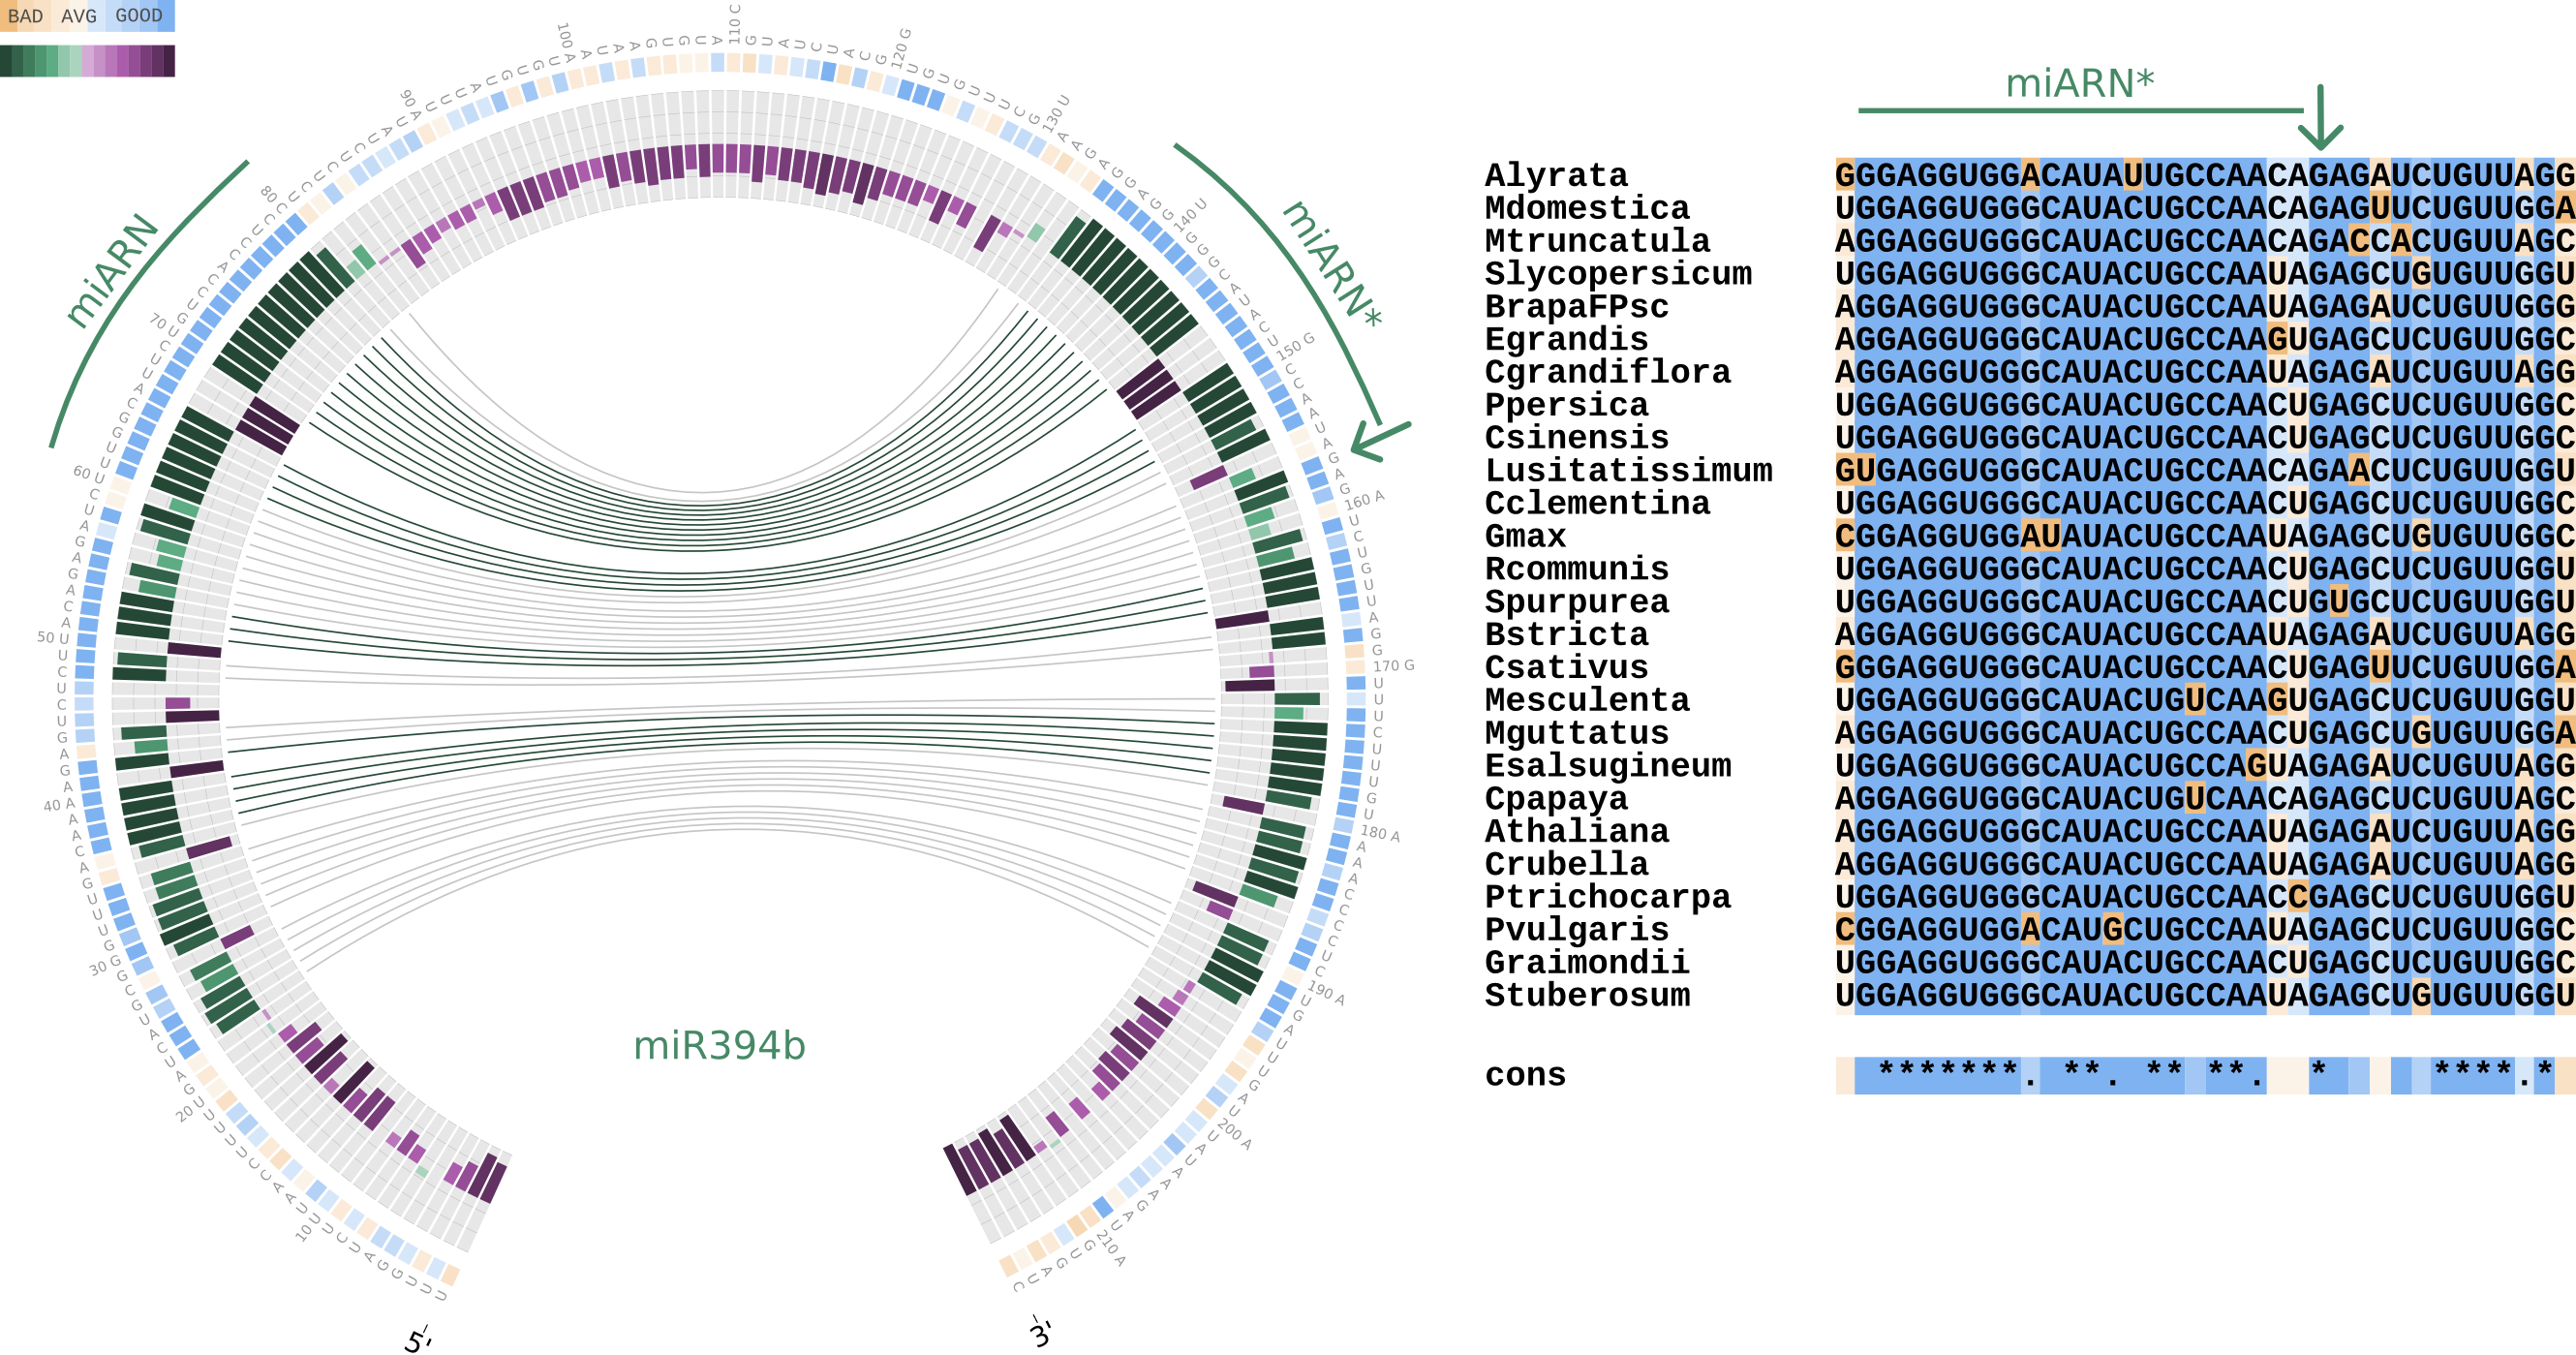
\includegraphics[width=.9\linewidth]{miR394b_circos.png}
	  \caption{Precursor del miR394b}
	  \label{subfig:miR394b_circos}
	\end{subfigure}
	\caption{Circos de precursores con mecanismos de procesamientos secuenciales de base a loop}
	\label{fig:seqBTL_circos}
	\end{figure}
\end{landscape}


\subsection{Mecanismo de loop a base cortos}

En los precursores con un mecanismo \textbf{cortos de loop a base}, el procesamiento es guiado por un tallo superior, y son necesarios dos cortes para liberar el miARN maduro.
La región terminal de estos precursores tienen una largo conservado de $\sim$42, donde incluye un loop pequeño \citep{Bologna2013} a diferencia de los precursores procesados dee base a loop, donde esta región es variable en tamaño.
Realizamos los Circos para precursores que se procesan cortos de base a loop y observamos que presentan una región conservada que corresponde al tallo superior, además de la región que comprende al dúplex miARN/miARN* (Figura \ref{fig:seqBTL_circos}).
A diferencia de los precursores que se procesan de la base al loop, estos precursores no presentan el tallo inferior ni estructurado ni conservado y esto se ve en los ejemplos del miR157a (Figura \ref{subfig:miR157a_circos}) y del miR160a (Figura \ref{subfig:miR157a_circos}).


\begin{landscape}
	\begin{figure}
	\centering
	\begin{subfigure}{.75\textwidth}
	  \centering
	  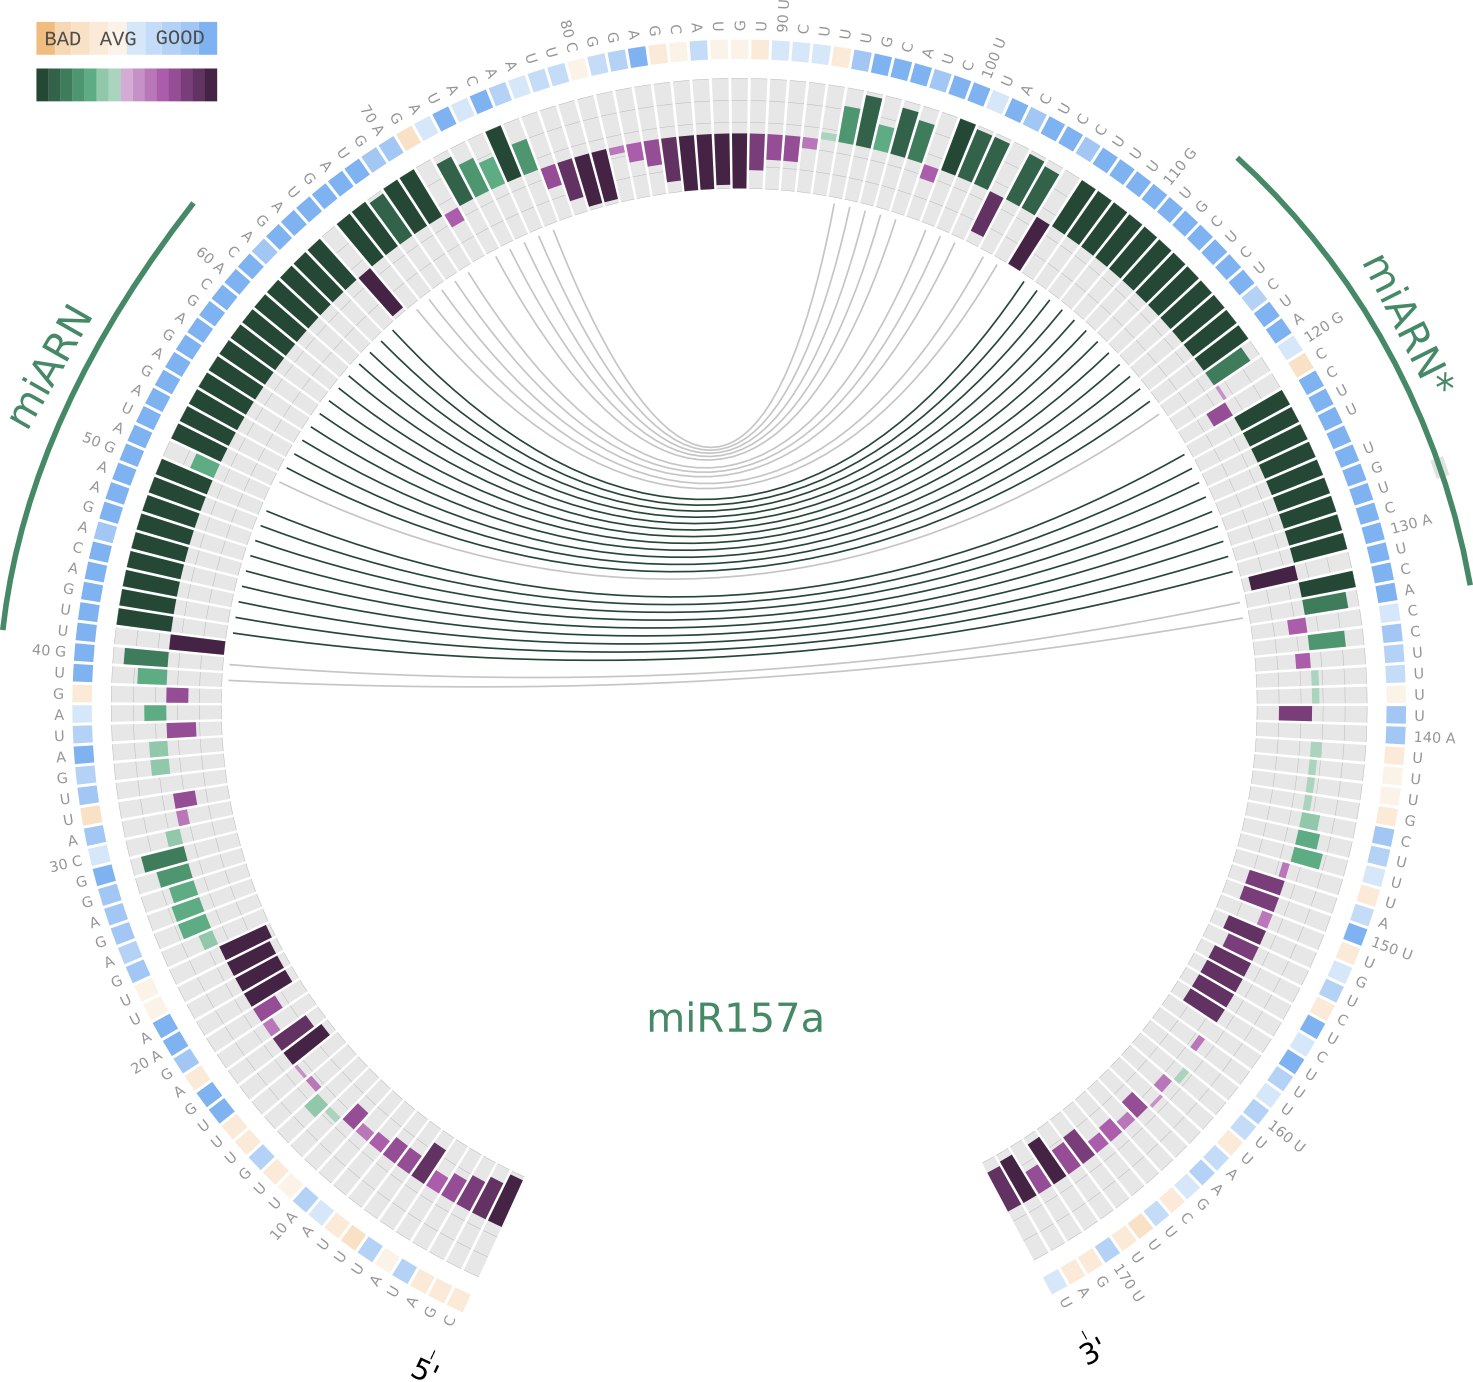
\includegraphics[width=.9\linewidth]{miR157a_circos.png}
	  \caption{Precursor del miR157a}
	  \label{subfig:miR157a_circos}
	\end{subfigure}%
	\begin{subfigure}{.75\textwidth}
	  \centering
	  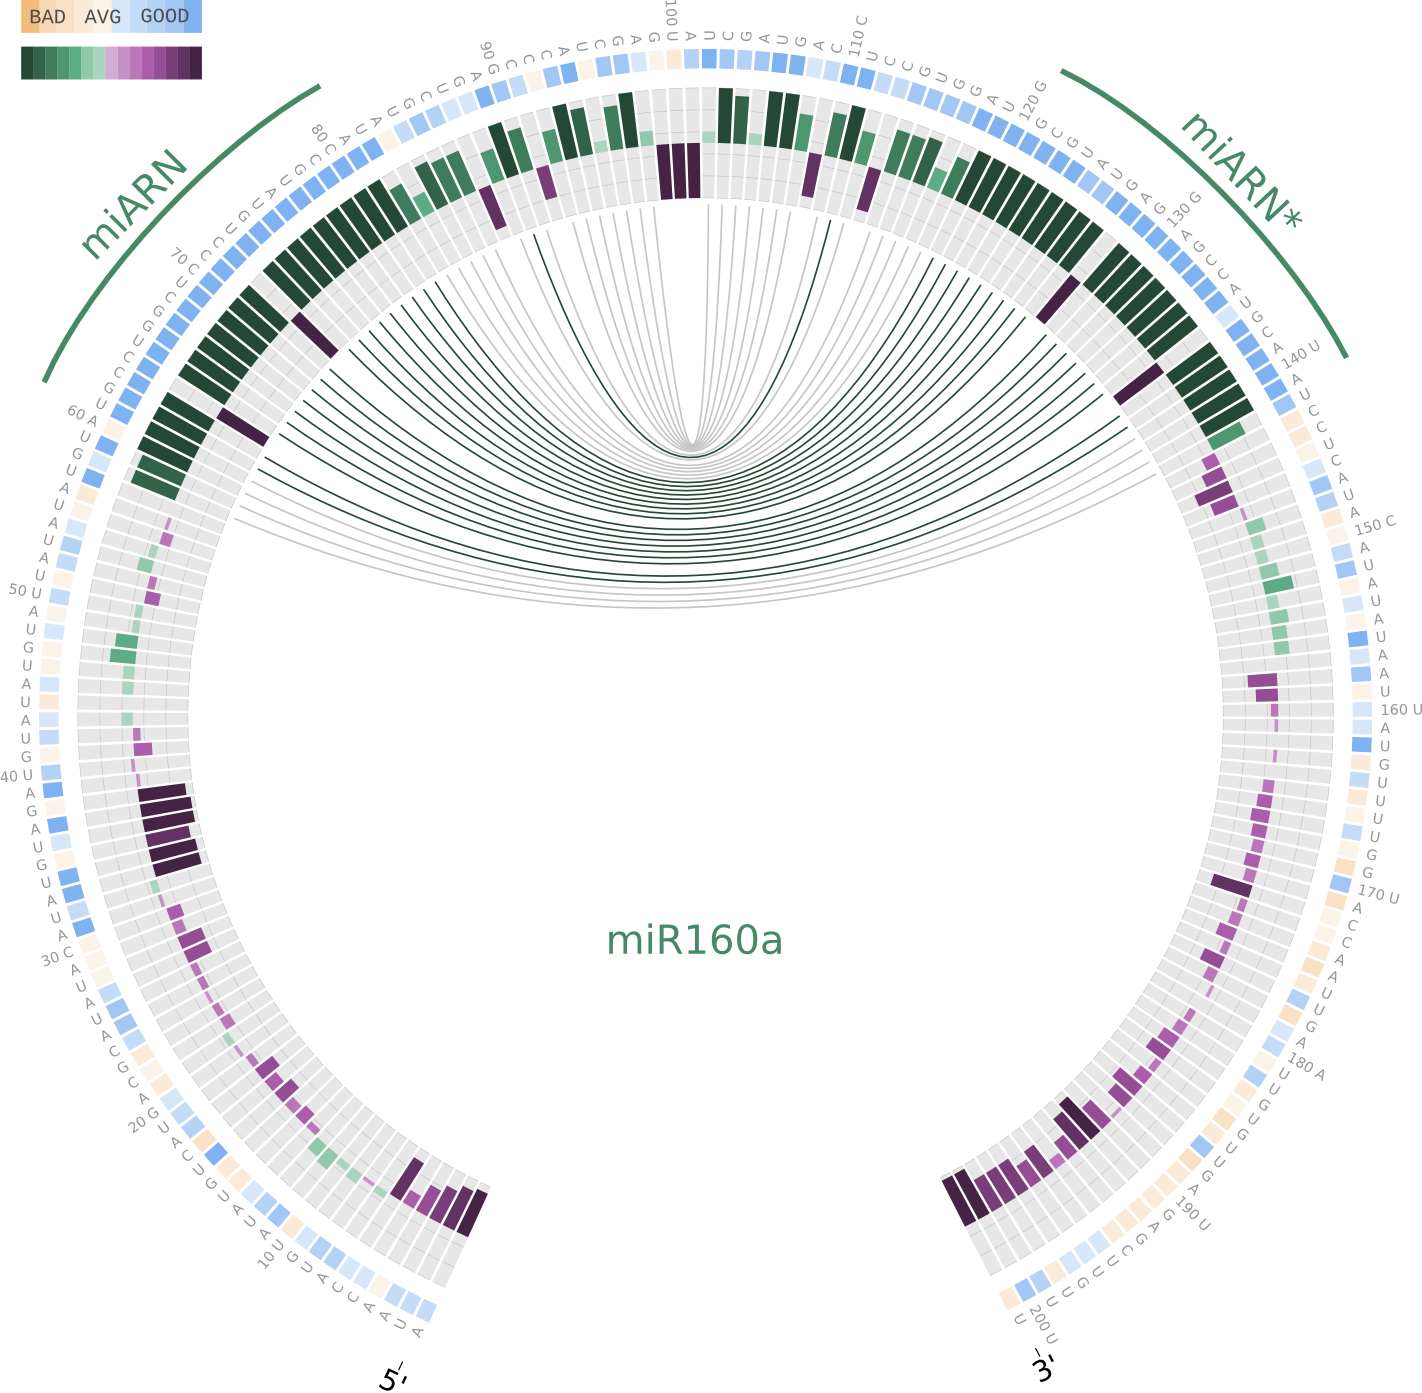
\includegraphics[width=.9\linewidth]{miR160a_circos.png}
	  \caption{Precursor del miR160a}
	  \label{subfig:miR160a_circos}
	\end{subfigure}
	\caption{Circos de precursores con mecanismos de procesamientos cortos de loop a base}
	\label{fig:srLTB_circos}
	\end{figure}
\end{landscape}

\subsection{Mecanismo de loop a base secuenciales}

En los precursores con un mecanismo \textbf{secuencial de loop a base}, cuatro cortes secuenciales por DCL1 son los encargados de procesar los precursores de miARNs.
En general, estos precursores muestran un tallo largo superior, del cual otros ARNs pequeños son generados \citep{pmid19850910,Bologna2009,Bologna2013}.

En este caso estudiamos la familia del miR319 y del miR159 y en particular mostramos al miR319a (Figura \ref{subfig:miR319a_circos}) y al miR159b (Figura \ref{subfig:miR159b_circos}).
Pudimos reconocer el tallo superior conservado y estructurado.
Además se pudo observar que los ARNs pequeños, que se originan del procesamiento de estos precursores, están conservados de la misma manera que el miARN y el miARN* (Figura \ref{fig:seqLTBL_circos}).

\begin{landscape}
	\begin{figure}
	\centering
	\begin{subfigure}{.75\textwidth}
	  \centering
	  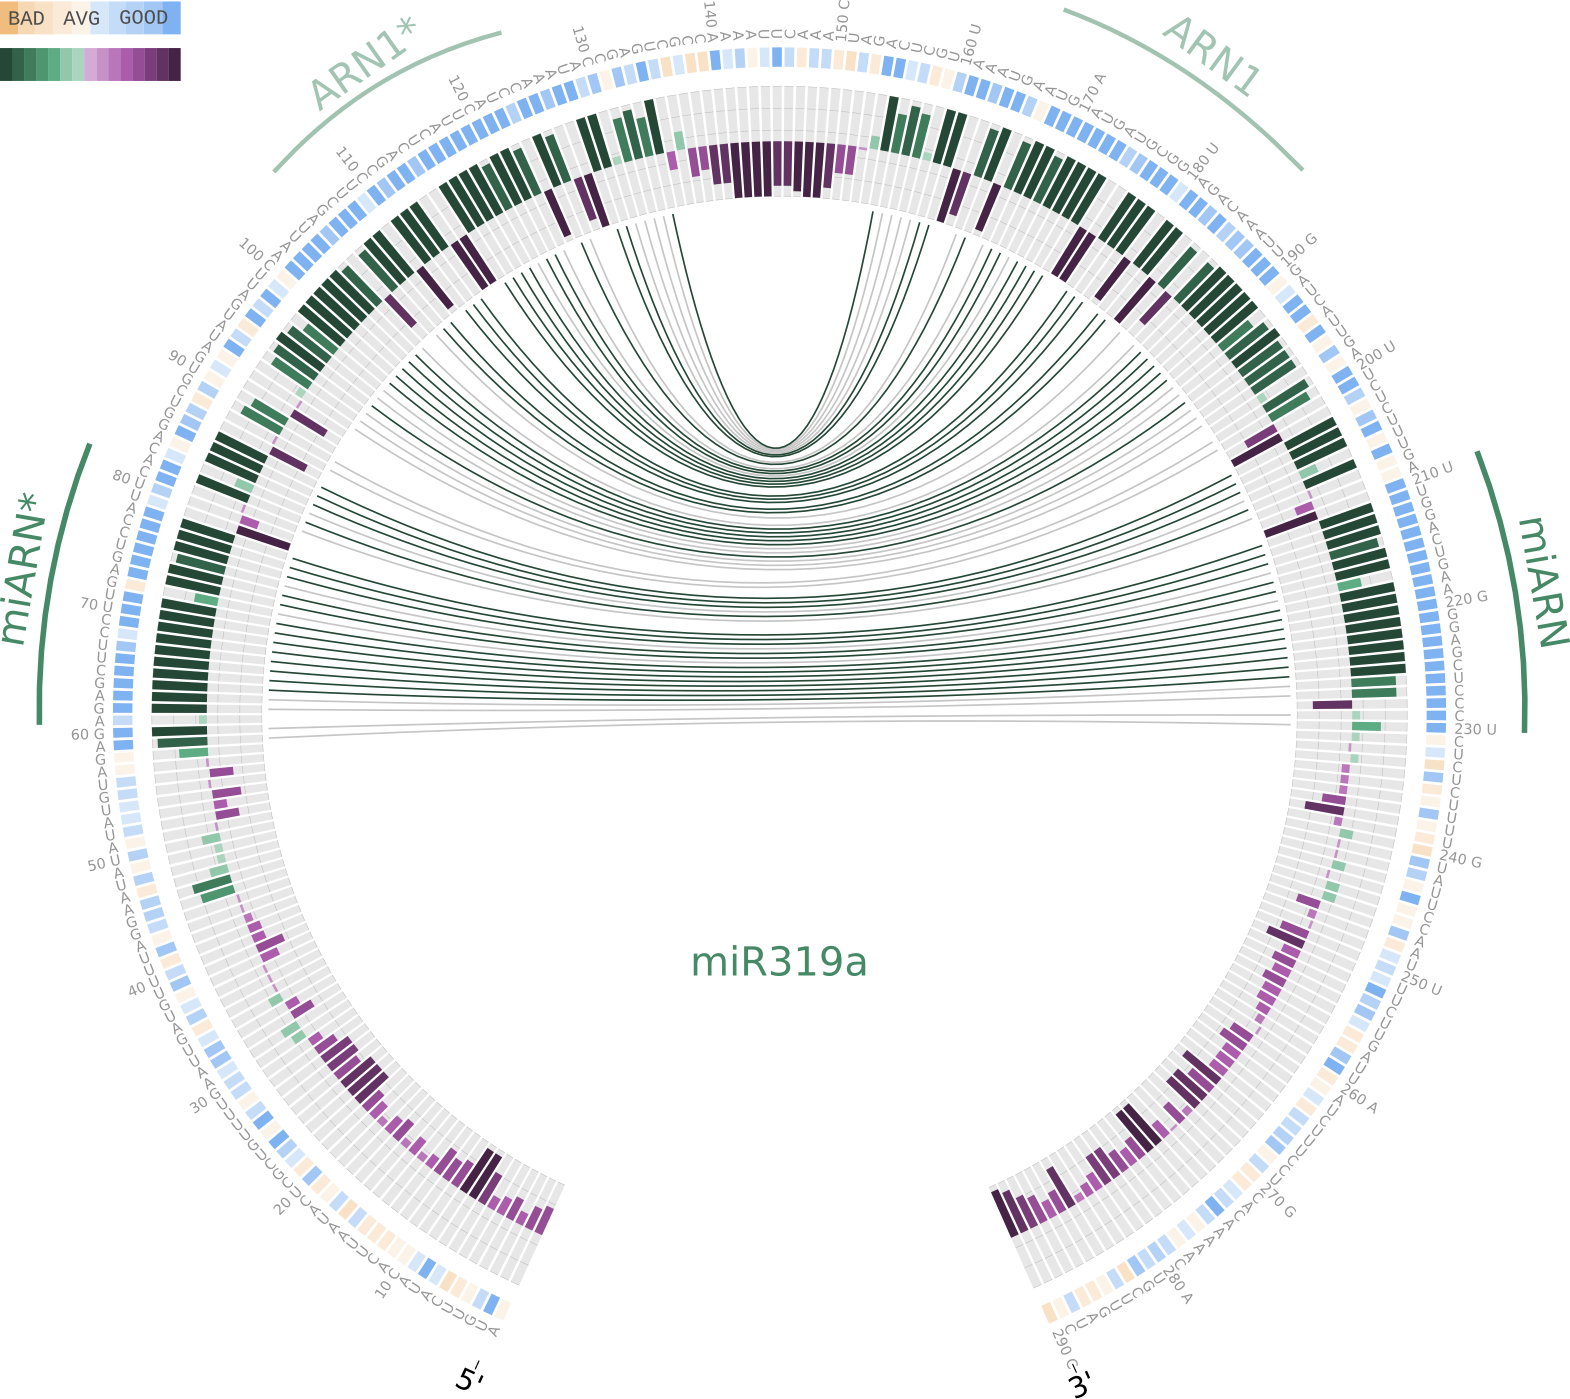
\includegraphics[width=.9\linewidth]{miR319a_circos.png}
	  \caption{Precursor del miR319a}
	  \label{subfig:miR319a_circos}
	\end{subfigure}%
	\begin{subfigure}{.75\textwidth}
	  \centering
	  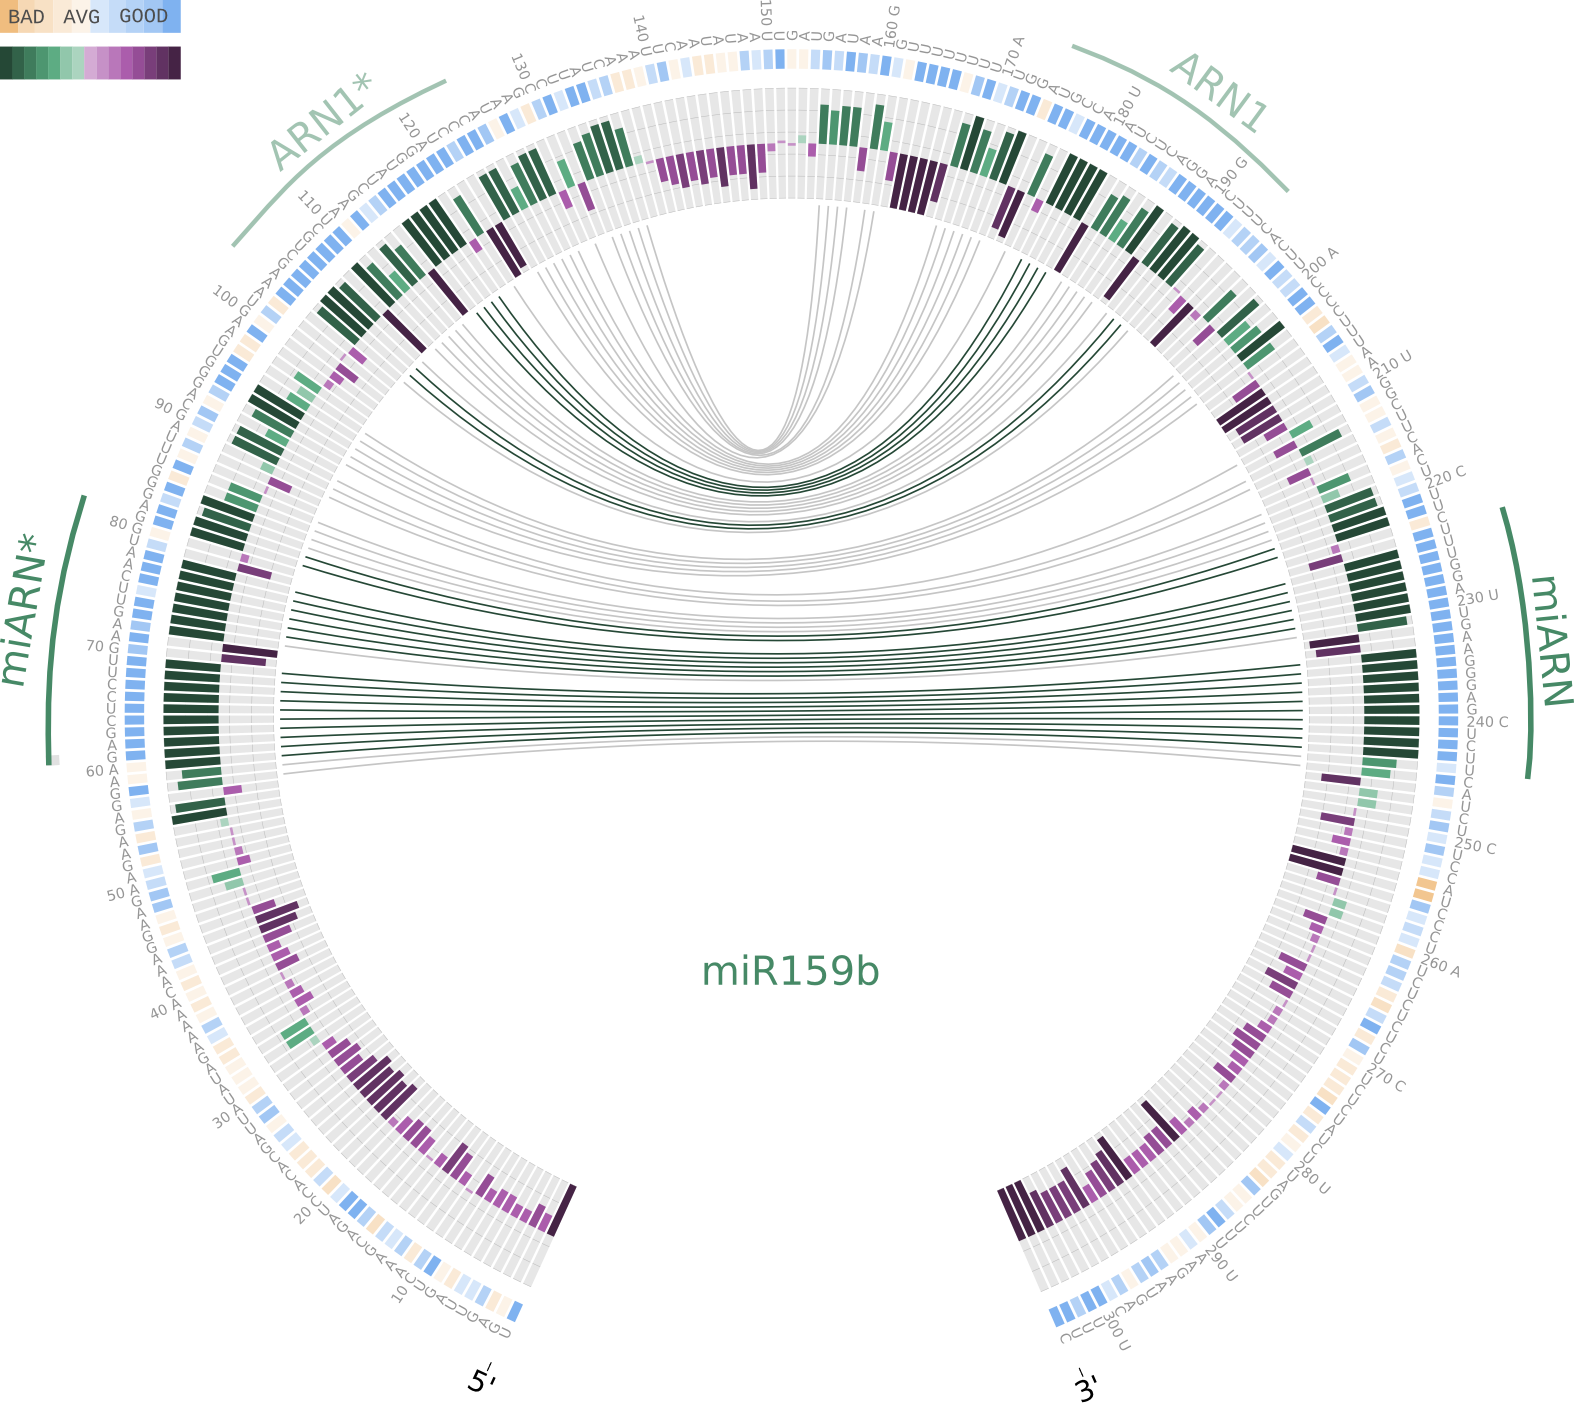
\includegraphics[width=.9\linewidth]{miR159b_circos.png}
	  \caption{Precursor del miR159b}
	  \label{subfig:miR159b_circos}
	\end{subfigure}
	\caption{Circos de precursores con mecanismos de procesamientos secuenciales de loop a base}
	\label{fig:seqLTBL_circos}
	\end{figure}
\end{landscape}


\subsection{Procesamiento mixto de miembros de la familia del miR171}

En general, se sabe que diferentes miembros de una misma familia de miARNs comparten la misma vía de biogenésis. 
Esta observación no sorprende ya que se cree que las familias de miARNs se expanden por eventos de duplicación de un gen ancestral \citep{pmid15565108}.
Sin embargo, ciertos el procesamiento de miembros de ciertas familias pueden variar de uno a otro \citep{Bologna2013}.
Esto sucede, por ejemplo,en la familia del miR171 donde en \textit{A. thaliana} existen 4 miembros. 
El precursor del miR171a es procesado de base a loop, mientras que los precursores del miR171b y miR171c son procesados de loop a base.

Nos pusimos analizar esta familia en detalle para ver si los patrones de conservación y estructura secundaria eran diferentes o no.


%~ Por otro lado, se seleccionaron todos los precursores que codifican para miARNs de la misma familia y luego los analizamos en conjunto.

